% IEEE Transactions on Medical Imaging — MIC v3
% Compile: pdflatex -> bibtex -> pdflatex -> pdflatex
\documentclass[journal]{IEEEtran}

% ---- Math / fonts ----
\usepackage{amsmath}
\usepackage{amssymb}
\usepackage{amsthm}

% ---- Graphics / tables ----
\usepackage{graphicx}
\usepackage{booktabs}
\usepackage{array}
\usepackage{multirow}

% ---- Utilities ----
\usepackage{xcolor}
\usepackage{url}
\usepackage{hyperref}
\usepackage{microtype}
\usepackage{listings}
\usepackage{algorithm}
\usepackage{algpseudocode}
\usepackage{caption}
\usepackage{subcaption}
\usepackage{cite}

\hypersetup{
  colorlinks=true,
  linkcolor=blue!70!black,
  citecolor=green!50!black,
  urlcolor=blue!70!black,
}

\lstset{
  basicstyle=\ttfamily\small,
  breaklines=true,
  columns=fullflexible,
}

% --------------------------------------------------
\title{A 16-Bit-Native Entropy Coding Pipeline for\\
       Lossless Medical Image Compression}

\author{Kuldeep~Singh%
\thanks{K.\ Singh is with Innovaccer Inc.
E-mail: kuldeep.singh@innovaccer.com.
Code: \url{https://github.com/pappuks/medical-image-codec}.}%
}

\markboth{IEEE Transactions on Medical Imaging,~Vol.~XX,~No.~XX,~2026}%
{Singh: A 16-Bit-Native Entropy Coding Pipeline}

% --------------------------------------------------

\begin{document}
\maketitle

% ============================================================
\begin{abstract}
Lossless compression remains important in medical imaging because archival
storage, transmission, and diagnostic workflows often require exact
reconstruction of high-bit-depth pixel data. Many medical images are stored at
10--16 bits per sample, yet most practical compression software remains
optimized for byte-oriented processing or small symbol alphabets. This paper
studies a lossless compression pipeline designed to operate natively on
predicted 16-bit residuals.

We present MIC, a codec consisting of three stages: spatial prediction, 16-bit
run-length encoding, and large-alphabet table-based asymmetric numeral system
(ANS) coding. The implementation extends FSE-style entropy coding to support
large active symbol sets arising in medical image residual streams and includes
a multi-state interleaved decoder that increases instruction-level parallelism
during decompression. The design is motivated by the observation that, after
simple spatial prediction, many medical images produce residual distributions
sharply concentrated near zero with frequently repeated 16-bit residual values.

We evaluate the proposed codec on 21 de-identified DICOM images spanning MR,
CT, CR, X-ray, mammography, nuclear medicine, radiography, secondary capture,
and fluoroscopy. On the evaluated dataset, the 16-bit-native pipeline improves
compression ratio by 5--22\% (geometric mean $+$14\%) relative to a
delta\,+\,Zstandard baseline, and its geometric mean ratio (3.12$\times$)
is within 1\% of HTJ2K (3.15$\times$) while being structurally simpler.
Across grayscale images, MIC achieves lossless
compression ratios ranging from 1.7$\times$ to 8.9$\times$. A four-state
interleaved entropy decoder provides 66--142\% decompression speedup over a
single-state implementation without affecting compressed size. On the reported
ARM64 and AMD64 platforms, the fastest MIC variant exceeds HTJ2K decompression
speed on 19/21 images single-threaded (ARM64) and 16/21 (AMD64);
strip-parallel configurations exceed HTJ2K on all 21 images on both platforms.

A compact JavaScript implementation (${\sim}$20\,KB, zero dependencies) and a
Go WebAssembly build demonstrate that the core decoding pipeline is lightweight
enough for client-side web deployment (i.e., in-browser decoding directly from
object storage, with no server-side transcoding). These results suggest that 16-bit-native
entropy coding is a useful design point for lossless medical image compression
when decompression throughput, implementation simplicity, and deployment
portability are important.
\end{abstract}

\begin{IEEEkeywords}
medical image compression, lossless compression, entropy coding, ANS, FSE,
DICOM, high-bit-depth imaging.
\end{IEEEkeywords}

% ============================================================
\section{Introduction}
\label{sec:intro}

\IEEEPARstart{M}{edical} imaging systems routinely generate large volumes of
high-bit-depth data. Modalities such as computed tomography (CT), magnetic
resonance imaging (MR), digital radiography (CR/XR), mammography, and
tomosynthesis commonly store pixel values at 10, 12, or 16 bits per sample. A
single digital breast tomosynthesis (DBT) acquisition view produces 60 or more
reconstructed slices---e.g., 69 frames at $2457 \times 1890$ pixels, 10-bit
depth---totalling over 600\,MB of raw pixel data per view. A complete bilateral
four-view screening study exceeds 2\,GB uncompressed. Efficient lossless
compression is essential for archival storage, network transmission, and
real-time rendering in clinical PACS and diagnostic viewers.

DICOM supports several established lossless transfer syntaxes, including
JPEG~2000, HTJ2K, JPEG-LS, and RLE Lossless. These methods offer different
tradeoffs among compression ratio, decoding speed, and implementation
complexity. JPEG~2000 and HTJ2K provide strong compression performance but rely
on transform and block-coding pipelines that are comparatively complex. JPEG-LS
uses predictive coding and often yields strong lossless ratios, but its
throughput characteristics remain application-dependent. RLE Lossless is simple
but typically provides limited compression because it operates on byte-oriented
runs and does not include an effective decorrelation stage.

This work studies a different design point for lossless medical image
compression: direct coding of \textbf{predicted 16-bit residual streams}.
Throughout this paper, a \emph{residual stream} denotes the sequence of
per-pixel prediction errors $r_{i,j} = x_{i,j} - \hat{x}_{i,j}$ produced by a
spatial predictor, kept at the native 16-bit precision of the source pixels
rather than re-serialised into bytes. In medical imaging these residuals are
typically sharply peaked at zero with long but sparse tails, and individual
16-bit residual values recur frequently---properties that motivate a
16-bit-native run-length and entropy coding stage. The
central observation is that the dominant entropy coders in modern compression
systems---Huffman, arithmetic coding, LZ77, and FSE/ANS as used in
Zstandard---were designed for 8-bit byte streams. Medical images break this
assumption: DICOM stores pixels at 10--16 bits per sample, yielding symbol
alphabets of 1,024 to 65,536 entries. Even after spatial delta prediction, the
residual alphabet for a 16-bit CT image can span tens of thousands of distinct
values. An entropy coder that assumes an 8-bit alphabet must either re-encode
16-bit symbols as byte pairs (losing inter-byte correlation and doubling the
number of coding steps) or truncate the alphabet at 256 and fall back to raw
storage for rare symbols. This mismatch is not merely inconvenient but
structurally costly: byte-splitting a 16-bit residual distribution discards
mutual information between the high and low bytes, inflating compressed output
by 10--22\% compared to a 16-bit-native entropy coder.

Based on this observation, we present MIC, a lossless codec that combines:
\begin{enumerate}
  \item a simple spatial predictor,
  \item a 16-bit-native run-length representation of the residual stream, and
  \item an extended FSE/tANS entropy coder supporting large active symbol
  alphabets.
\end{enumerate}

The codec also includes multi-state interleaved entropy decoding to improve
decompression throughput by increasing instruction-level parallelism.

The paper is motivated by three practical questions:
\begin{enumerate}
  \item Can a 16-bit-native entropy coding pipeline improve compression
  efficiency over byte-oriented baselines on medical residual streams?
  \item Can entropy-decoder organization be modified to improve throughput
  without changing compressed size?
  \item Can such a codec remain compact enough for lightweight deployment,
  including client-side decoding?
\end{enumerate}

\subsection{Contributions}

The main contributions of this paper are as follows.

\begin{enumerate}
  \item \textbf{A 16-bit-native lossless coding pipeline for medical images.}
  We present a Delta\,+\,16-bit RLE\,+\,extended FSE pipeline for grayscale
  medical image compression that outperforms Delta\,+\,Zstandard by 5--22\%
  (geometric mean $+$14\%) on all 21 tested images.

  \item \textbf{An extended table-based entropy coder for large residual
  alphabets.}
  The proposed implementation supports up to 65,535 distinct symbols while
  dynamically sizing working tables to the observed symbol range, reducing
  working-set size from 512\,KB to approximately 2\,KB for 8-bit images.

  \item \textbf{A multi-state interleaved entropy decoder.}
  We implement and evaluate two-state and four-state FSE decoding to exploit
  instruction-level parallelism, achieving 66--142\% isolated FSE speedup with
  no compression ratio penalty.

  \item \textbf{An empirical evaluation against standard codecs and a
  general-purpose baseline.}
  We compare MIC with HTJ2K (OpenJPH)~\cite{openjph}, JPEG-LS
  (CharLS)~\cite{charls}, and delta\,+\,Zstandard on a dataset of 21 public
  de-identified DICOM images spanning 10 modalities, using fair in-process
  benchmarking via CGO bindings.

  \item \textbf{A compact JavaScript/WASM decoder implementation.}
  We provide a ${\sim}$20\,KB pure JavaScript decoder and a Go WebAssembly
  build to explore deployment feasibility for client-side viewing.
\end{enumerate}

\subsection{Scope}

The primary focus of this paper is \textbf{lossless grayscale medical image
compression}. Multi-frame grayscale (MIC2) and single-frame RGB support (MICR)
are included as secondary studies demonstrating extensibility. The present work
does not address lossy coding, progressive decoding, or region-of-interest
coding.

\subsection{Organization}

Section~\ref{sec:related} reviews related work and positions MIC relative to
existing methods. Section~\ref{sec:pipeline} describes the proposed coding
pipeline. Section~\ref{sec:multistate} presents the multi-state entropy decoder.
Section~\ref{sec:methodology} describes experimental methodology.
Section~\ref{sec:results} reports compression and speed results.
Section~\ref{sec:discussion} discusses limitations and implications.
Section~\ref{sec:conclusion} concludes.

% ============================================================
\section{Related Work}
\label{sec:related}

\subsection{Lossless Compression in Medical Imaging}

JPEG~2000 Part~1~\cite{taubman2002} employs the reversible 5/3 integer wavelet
transform with embedded block coding (EBCOT). It achieves excellent compression
ratios but its bit-plane coding and context modeling impose significant
computational overhead during decompression. High-Throughput JPEG~2000
(HTJ2K)~\cite{htj2k2019} replaces EBCOT with a faster block coder,
substantially improving decode speed while maintaining JPEG~2000 compatibility.

JPEG-LS~\cite{loco1} uses context-adaptive prediction (MED predictor) followed
by Golomb-Rice coding. It provides fast encoding and decoding with strong
compression ratios---in our evaluation, JPEG-LS achieves the highest lossless
ratio on 21/21 tested images. JPEG-LS is well-suited to smooth images but its
prediction model is fixed and its throughput characteristics are
application-dependent.

RLE Lossless (DICOM Transfer Syntax 1.2.840.10008.1.2.5) uses byte-level
PackBits run-length encoding. It is trivially simple but achieves poor
compression ratios (typically $<$1.5$\times$) because it operates on bytes
rather than 16-bit pixel values and lacks any decorrelation stage.

These standards are important baselines for the present work. The goal of this
paper is not to argue that they are obsolete, but to investigate a simpler
residual-domain design targeted specifically at high-bit-depth images with
strong throughput characteristics.

\subsection{Entropy Coding and the Byte Assumption}

Asymmetric numeral systems (ANS)~\cite{duda2009,duda2013} generalize arithmetic
coding into a single-state machine that replaces interval subdivision with
integer state transitions. Finite State Entropy (FSE)~\cite{fse} is a
table-driven tANS implementation that achieves near-optimal compression with
$\mathcal{O}(1)$ per-symbol operations. FSE was popularized by
Zstandard~\cite{rfc8878}. Recent theoretical analyses have formalized ANS
efficiency bounds~\cite{kosolobov2022} and provided statistical
interpretations~\cite{bamler2022}.

Traditional arithmetic coding achieves near-optimal compression but is
inherently sequential. Mahapatra and Singh~\cite{mahapatra2007} addressed this
with a parallel-pipelined FPGA implementation, demonstrating that hardware
acceleration can overcome the throughput limitations of sequential arithmetic
coders.

In practice, most of these coders are designed around small alphabets. Huffman
coding becomes impractical above ${\sim}$4,096 symbols. FSE in Zstandard caps
at 4,096. The predominant implementations are optimized for byte-oriented data.

Medical images differ in that they naturally contain 10--16 bit sample values.
After prediction, the residual stream may still be more naturally modeled as a
sequence of 16-bit symbols. This creates a modeling choice: preserve the
residual stream as word-level symbols, or transform it into bytes and rely on
later processing to recover cross-byte structure.

\textbf{The information-theoretic cost of byte-splitting.} Consider a 16-bit
symbol $X$ decomposed into its high byte $X_H$ and low byte $X_L$. A byte-level
coder that processes $X_H$ and $X_L$ independently achieves at best
$H(X_H) + H(X_L) = H(X) + I(X_H;\, X_L)$, where $I(X_H;\, X_L)$ is the
mutual information between the two bytes. For medical image residuals after
delta prediction, when a residual is small (say, $\pm 30$), the high byte is
nearly deterministic given the low byte---yet a byte-level coder must still
encode it. On our test images, $I(X_H;\, X_L)$ ranges from 0.3\,bits/symbol
(MR) to 1.1\,bits/symbol (MG3), corresponding to 8--22\% of the total entropy
and closely matching the 5--22\% empirical advantage of MIC over
Delta\,+\,Zstandard (geometric mean $+$14\%).

\subsection{ANS and Interleaved Decoding}

Prior work has shown that interleaving or multi-stream organization can improve
ANS decoder throughput. Giesen~\cite{giesen2014,giesen2014b} demonstrated the
value of multi-stream rANS; Lin~\textit{et al.}~\cite{lin2023} extended parallel
rANS to decoder-adaptive scalability; Weissenberger and
Schmidt~\cite{weissenberger2019} showed massively parallel ANS decoding on
GPUs. The present work does not claim novelty in ANS itself or in interleaving
as a general concept. Rather, the contribution lies in applying these ideas in a
16-bit-native medical image codec, together with a specific large-alphabet
implementation and throughput-oriented software design.

\subsection{Positioning of This Work}

Table~\ref{tab:positioning} distinguishes MIC from prior work across five
dimensions relevant to medical image compression.

\begin{table}[htbp]
\centering
\caption{Feature comparison of MIC with related codecs and entropy coding
methods.}
\label{tab:positioning}
\scriptsize
\begin{tabular}{p{2.0cm}ccccc}
\toprule
Feature & JPEG-LS & HTJ2K & Zstd & rANS & MIC \\
\midrule
Lossless medical & Yes & Yes & Gen. & Gen. & Yes \\
Native 16-bit & No & No & No & Config. & Yes \\
Multi-state ILP & No & No & No & Yes & Yes \\
Browser decoder & No & No & Part. & No & Yes \\
Implementation size (LOC) & 5k & 20k & N/A & N/A & 1.1k \\
\bottomrule
\end{tabular}

\vspace{0.5em}
\footnotesize
Table~\ref{tab:positioning} contrasts MIC against four reference points along
dimensions that matter for a medical-imaging deployment: whether the codec is a
lossless medical image standard, whether it treats samples as 16-bit symbols
natively instead of splitting them into bytes, whether its decoder exposes
multiple state machines for instruction-level parallelism, whether a usable
in-browser decoder exists, and an order-of-magnitude estimate of the core
decoder implementation size in source lines of code (SLOC, excluding
build/test). JPEG-LS (CharLS) and HTJ2K (OpenJPH) are mature C/C++ codebases
of roughly 5k and 20k lines respectively; Zstandard and rANS are
general-purpose and do not ship as medical image codecs; MIC's core Delta +
RLE + FSE decoder is ${\sim}$1.1k lines of Go, is 16-bit-native by construction,
interleaves up to four FSE state machines, and ships a zero-dependency
JavaScript decoder for browsers.
\normalsize
\end{table}

% ============================================================
\section{Proposed Method}
\label{sec:pipeline}

MIC compresses grayscale images using three sequential stages: spatial
prediction, 16-bit run-length encoding, and large-alphabet table-based entropy
coding. Each stage is simple enough to decode in a single sequential pass with
minimal branching.

\begin{figure*}[tbp]
\centering
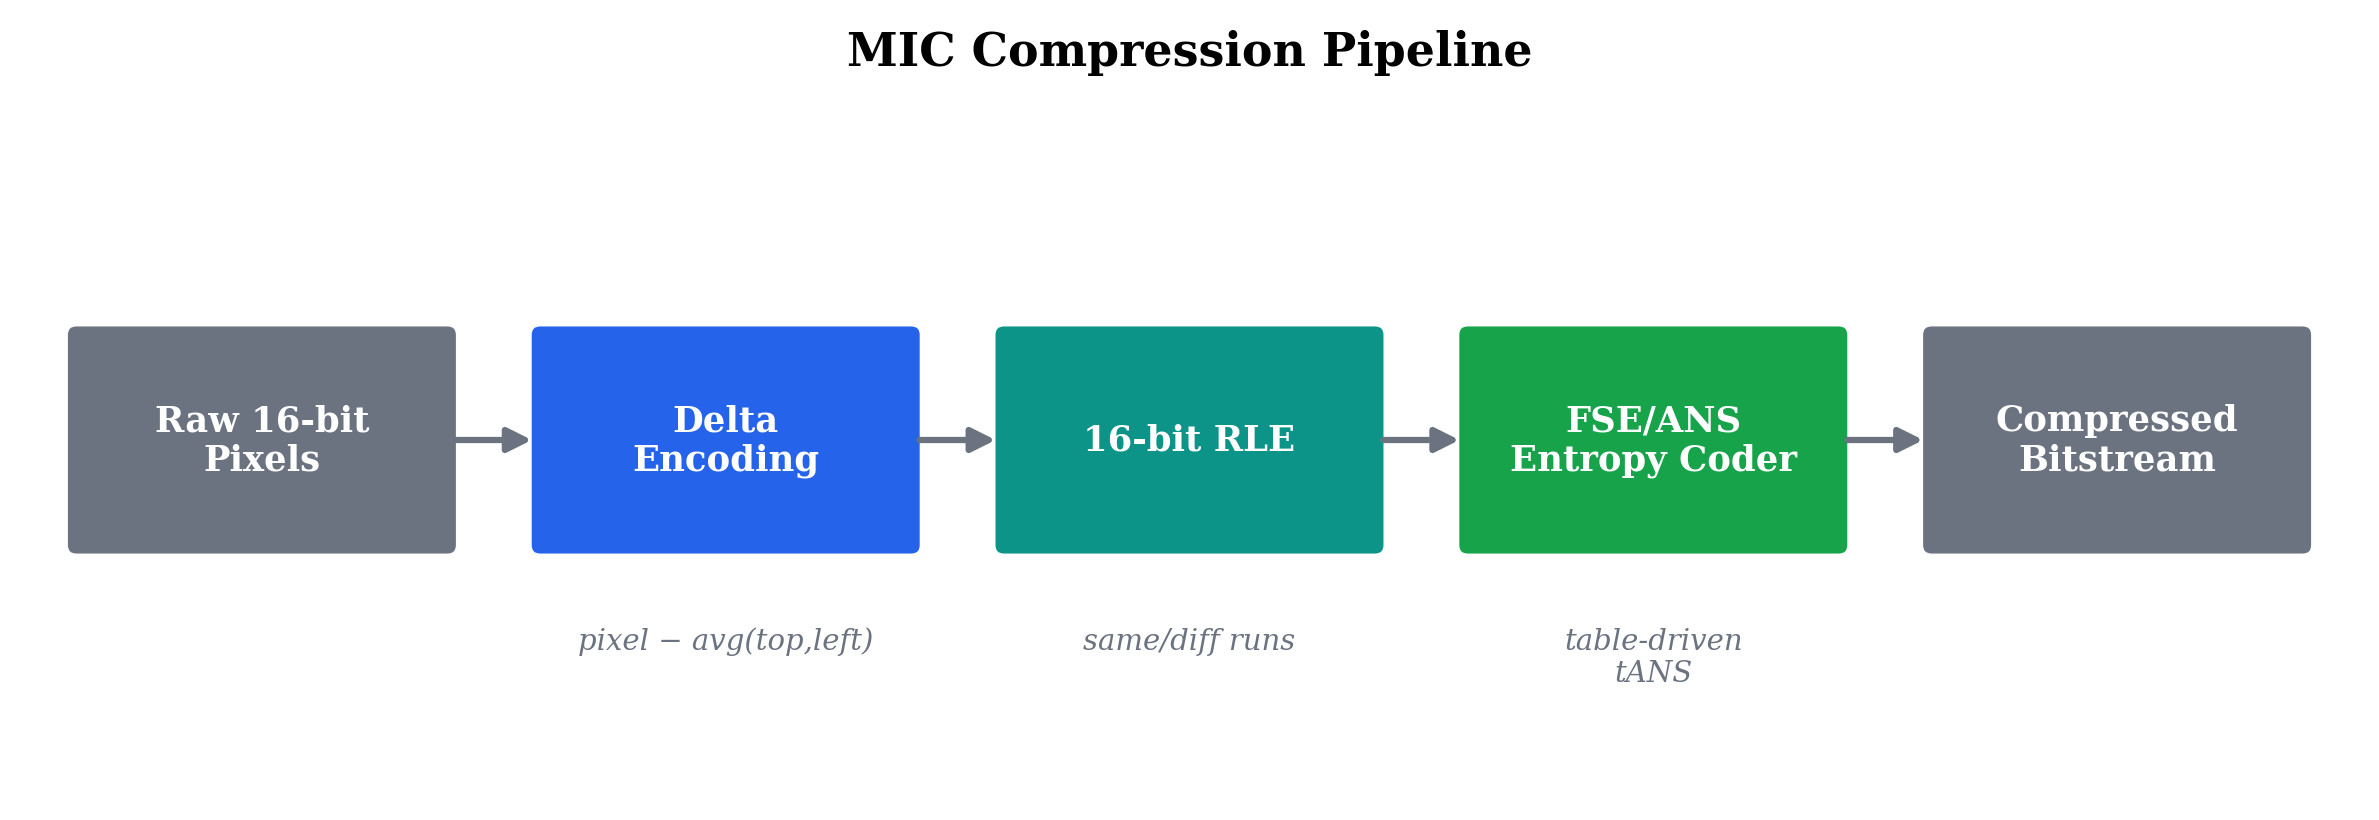
\includegraphics[width=0.85\textwidth]{figures/fig1_pipeline.png}
\caption{MIC compression pipeline---Raw 16-bit pixels are delta-encoded (avg of
top and left neighbors), run-length encoded (same/diff runs), and entropy-coded
with a 16-bit-native FSE/tANS coder.}
\label{fig:pipeline}
\end{figure*}

\subsection{Spatial Prediction}

Let $x_{i,j}$ denote the pixel at row $i$, column $j$. For interior pixels, MIC
predicts the current pixel from the average of the top and left neighbors:
\begin{equation}
  \hat{x}_{i,j} = \left\lfloor \frac{x_{i-1,j} + x_{i,j-1}}{2} \right\rfloor
\end{equation}
and forms the residual:
\begin{equation}
  r_{i,j} = x_{i,j} - \hat{x}_{i,j}.
\end{equation}

Boundary pixels use only the available neighbor, and the first pixel is stored
directly. This predictor was selected because it is computationally simple,
branch-light in decoding, and effective on the current dataset.

\textbf{Predictor comparison.} We implemented and compared four predictors
through the full RLE\,+\,FSE pipeline on the 21-image dataset: left-only (left
neighbor, no top), average (MIC default), Paeth (PNG predictor~\cite{png}), and
MED (JPEG-LS~\cite{loco1}). Table~\ref{tab:predictor-summary} summarizes
geometric means and relative gains.

\begin{table}[htbp]
\centering
\caption{Predictor ablation summary---geometric means and win counts across all
21 images.}
\label{tab:predictor-summary}
\begin{tabular}{lrrr}
\toprule
Predictor & Geo.\ Mean & Wins & Avg$\to$X \\
\midrule
Left-only & 3.38$\times$ & 3/21 & $-$2.3\% \\
Average (MIC) & 3.46$\times$ & 13/21 & baseline \\
Paeth & 3.48$\times$ & 2/21 & $+$0.5\% \\
MED (JPEG-LS) & 3.52$\times$ & 16/21 & $+$1.6\% \\
\bottomrule
\end{tabular}
\end{table}

MED decompression is 1.5--2$\times$ slower due to the three-way conditional
branch and diagonal neighbor dependency that prevents the branch-free interior
loop optimization used by the average predictor. The results show no single
predictor dominates. MED yields the best geomean ratio ($+$1.6\% over Avg) but
at significant speed cost. The average predictor is retained as the default
because its per-modality performance is more consistent and its decompression
path is branch-free.

\begin{figure*}[tbp]
\centering
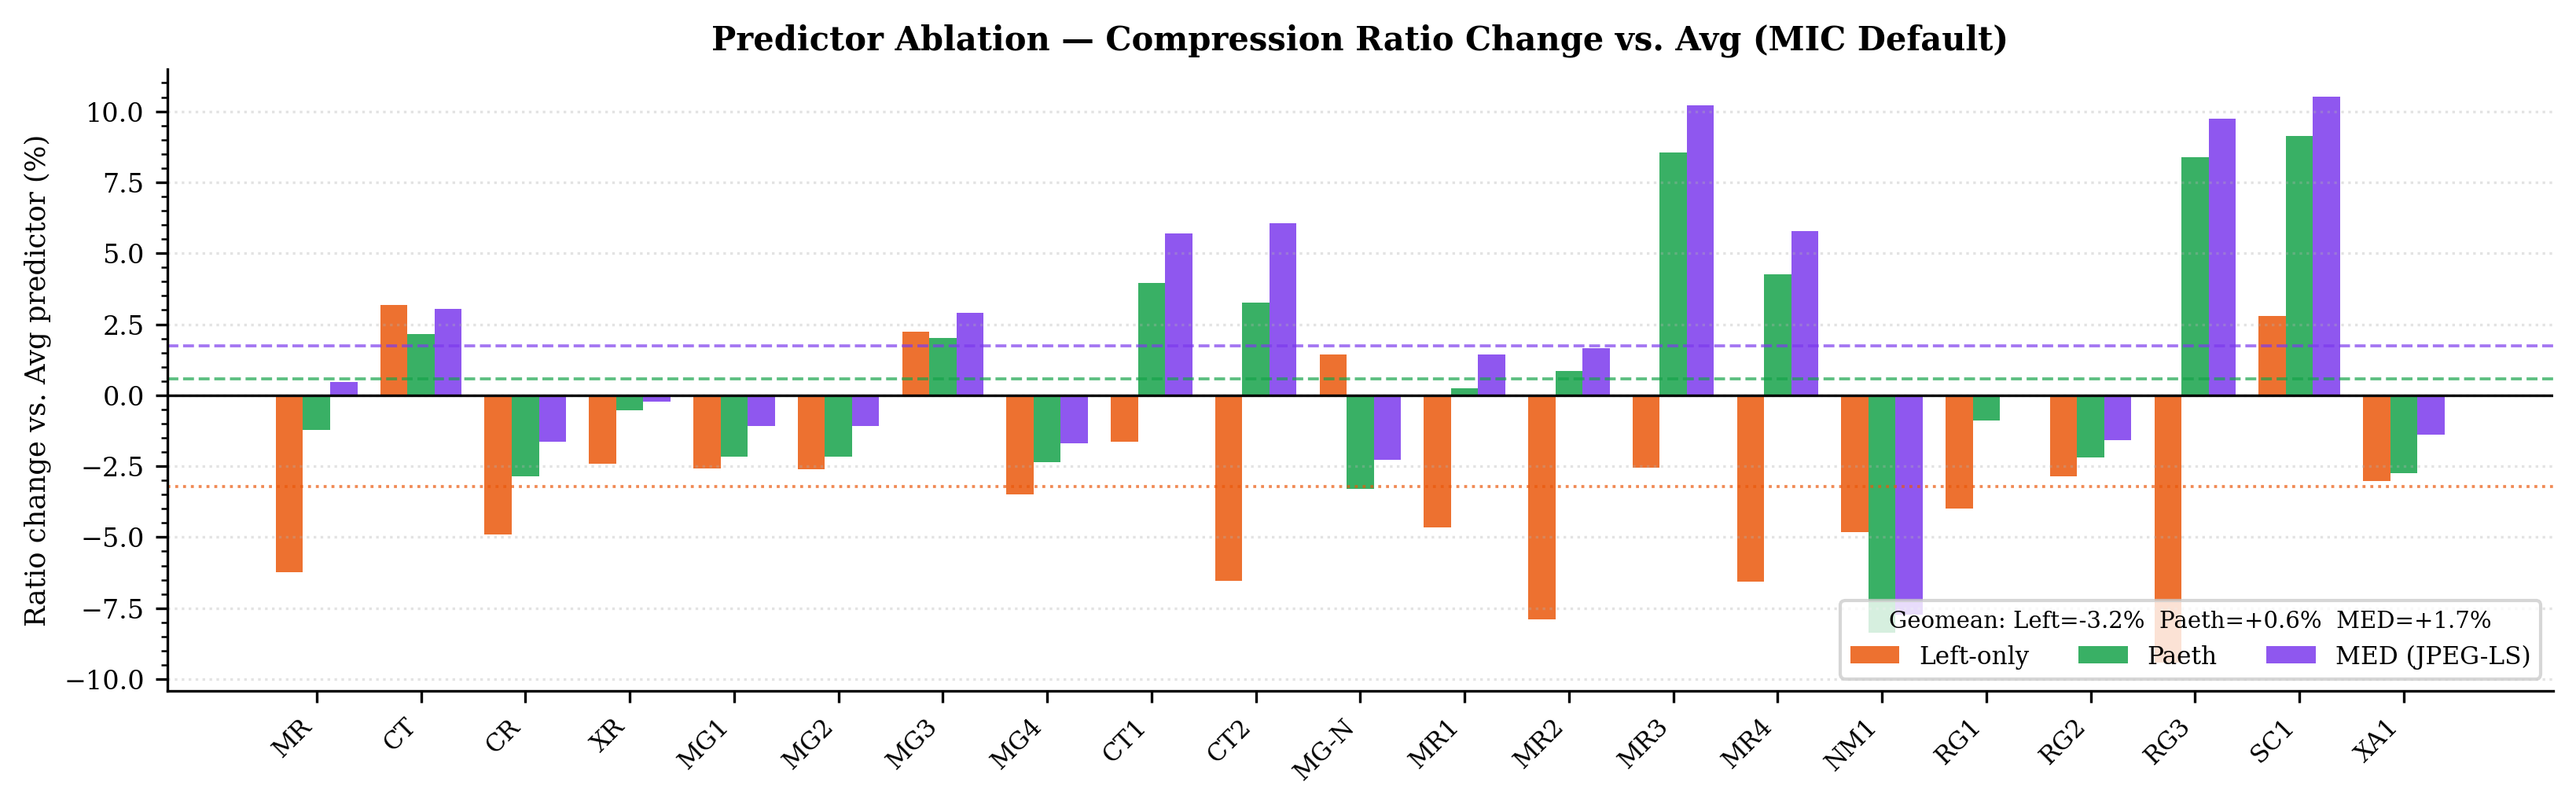
\includegraphics[width=0.85\textwidth]{figures/fig5_predictor_ablation.png}
\caption{Compression ratio change vs.\ Avg predictor for left-only, Paeth, and
MED, across all 21 images. Dashed lines show geomean for each predictor.}
\label{fig:predictor-ablation}
\end{figure*}

\subsection{Effective Bit Depth and Overflow Coding}

For 16-bit images, residuals can span $[-65535, +65535]$. Rather than widening
the main residual stream to 32 bits, MIC uses an overflow delimiter scheme
derived from the effective image bit depth:
\begin{equation}
  d = \lceil \log_2(\max(x) + 1) \rceil.
\end{equation}

Residuals within an in-range interval are mapped directly to 16-bit codes.
Residuals outside that interval are encoded using a delimiter followed by the
raw pixel value.

\textbf{Encoding procedure:}
\begin{enumerate}
  \item Compute \texttt{deltaThreshold} $= 2^{d-1} - 1$.
  \item Compute delimiter $D = 2^d - 1$.
  \item For each residual $r_{i,j}$: if $|r_{i,j}| <$ \texttt{deltaThreshold},
  emit \texttt{uint16(deltaThreshold $+$ $r_{i,j}$)}; otherwise emit delimiter
  $D$, then emit raw pixel $x_{i,j}$.
\end{enumerate}

\textbf{Non-collision proof.} In-range residuals satisfy $|r| \leq$
\texttt{deltaThreshold}~$-$~$1$, so stored values range from 1 to $2^d - 3$.
The delimiter is $D = 2^d - 1$. Since $2^d - 3 < 2^d - 1$, the stored value of
a direct residual can never equal $D$; the two ranges are disjoint.

\subsection{16-Bit Run-Length Encoding}

The predicted residual stream is converted into an alternating sequence of:
\begin{itemize}
  \item \textbf{Same runs}: a count and a repeated 16-bit value;
  \item \textbf{Diff runs}: a count followed by a sequence of distinct 16-bit
  values.
\end{itemize}

A same run is emitted only when at least three consecutive identical values are
observed. Run headers use a midpoint protocol: counts $\leq$ \texttt{midCount}
signal same runs; counts $>$ \texttt{midCount} signal diff runs.

\textbf{Why 16-bit RLE matters.} Consider a run of 1,000 identical non-zero
16-bit residuals, e.g.\ the value $v = \texttt{0x0103}$. MIC's 16-bit RLE
represents the entire run with two uint16 words---a count and the value
$v$---regardless of the byte pattern of $v$. A byte-oriented RLE applied to the
same data sees the interleaved stream $\texttt{0x01,0x03,0x01,0x03,\ldots}$
(little-endian: $\texttt{0x03,0x01,0x03,0x01,\ldots}$): there is no single
byte that repeats 1,000 times, so it must emit two interleaved byte runs of
length 1,000, or, if the two alternating byte values alias with the run
sentinel, fall back to literal bytes entirely. Only the special case $v = 0$
(or any value whose two bytes happen to be equal) collapses cleanly to a
single byte-level run. For generic 16-bit residuals the 16-bit-native
representation is structurally tighter by a factor of $\sim$2 on repeated
values, and this gap grows when the alternating byte pattern breaks a
byte-level RLE's run-detection heuristic entirely.

\textbf{Same-run fast path.} Same-value runs (often $>$80\% of all runs on
smooth medical images after delta coding) are fast-pathed in the decoder to
return the cached value without touching the compressed-data slice. Each output
symbol in a same run requires only a counter decrement.

\subsection{Large-Alphabet FSE Coding}

The RLE output is entropy-coded using table-based ANS (tANS), implemented as
Finite State Entropy. MIC extends FSE to support up to 65,535 distinct symbols
(versus the 4,095 limit in Zstandard).

\textbf{Encoding} processes symbols in reverse order (last symbol first),
building the compressed bitstream from the end. \textbf{Decoding} reads bits
forward, using a decode table indexed by current state. Each decode step
requires only a table lookup, a bit read, and an addition---no divisions or
multiplications.

\textbf{Dynamic table sizing.} Encode and decode tables are sized to the actual
observed symbol range rather than the theoretical 65,536 maximum. For 8-bit
images stored in 16-bit containers (common in MR), this reduces the working set
from 512\,KB to approximately 2\,KB.

\subsection{Adaptive Table Size Selection}

MIC automatically adjusts the FSE table log based on the number of active
symbols and the density of observations per symbol:
\begin{itemize}
  \item Default $\textit{tableLog} = 11$.
  \item Bumped to 12 when $\textit{symbolDensity} > 32$ and
  $\textit{symbolLen} > 128$.
  \item Bumped to 13 when $\textit{symbolLen} > 512$ and
  $\textit{symbolDensity} > 16$.
\end{itemize}
where $\textit{symbolDensity} = \textit{inputLength} / \textit{symbolLen}$.

Table~\ref{tab:tablelog-ablation} presents the tableLog ablation across
selected images.

\begin{table}[htbp]
\centering
\caption{TableLog ablation---forced TL=11/12/13 vs.\ adaptive selection
(selected images, Apple M2 Max).}
\label{tab:tablelog-ablation}
\scriptsize
\begin{tabular}{lrrrr}
\toprule
Image & TL=11 & TL=12 & TL=13 & Adaptive \\
\midrule
CR  & 3.47$\times$ & 3.63$\times$ & 3.69$\times$ & 3.69$\times$ \\
MG1 & 8.00$\times$ & 8.57$\times$ & 8.79$\times$ & 8.79$\times$ \\
MG2 & 7.98$\times$ & 8.55$\times$ & 8.77$\times$ & 8.77$\times$ \\
MR2 & 3.14$\times$ & 3.24$\times$ & 3.28$\times$ & 3.28$\times$ \\
RG2 & 3.85$\times$ & 4.12$\times$ & 4.23$\times$ & 4.23$\times$ \\
RG3 & 5.64$\times$ & 5.95$\times$ & 6.08$\times$ & 6.08$\times$ \\
\bottomrule
\end{tabular}
\end{table}

Nine images benefit from TL=12 or TL=13: CR ($+$6.3\%), MG1 ($+$9.9\%), MG2
($+$9.9\%), MR2 ($+$4.6\%), RG2 ($+$9.9\%), RG3 ($+$7.8\%), XA1 ($+$4.4\%),
MR3 ($+$0.9\%), NM1 ($+$1.9\%). The adaptive policy correctly identifies all
beneficial cases. Decompression throughput is unaffected by tableLog choice
($<$5\% variation).

\begin{figure*}[tbp]
\centering
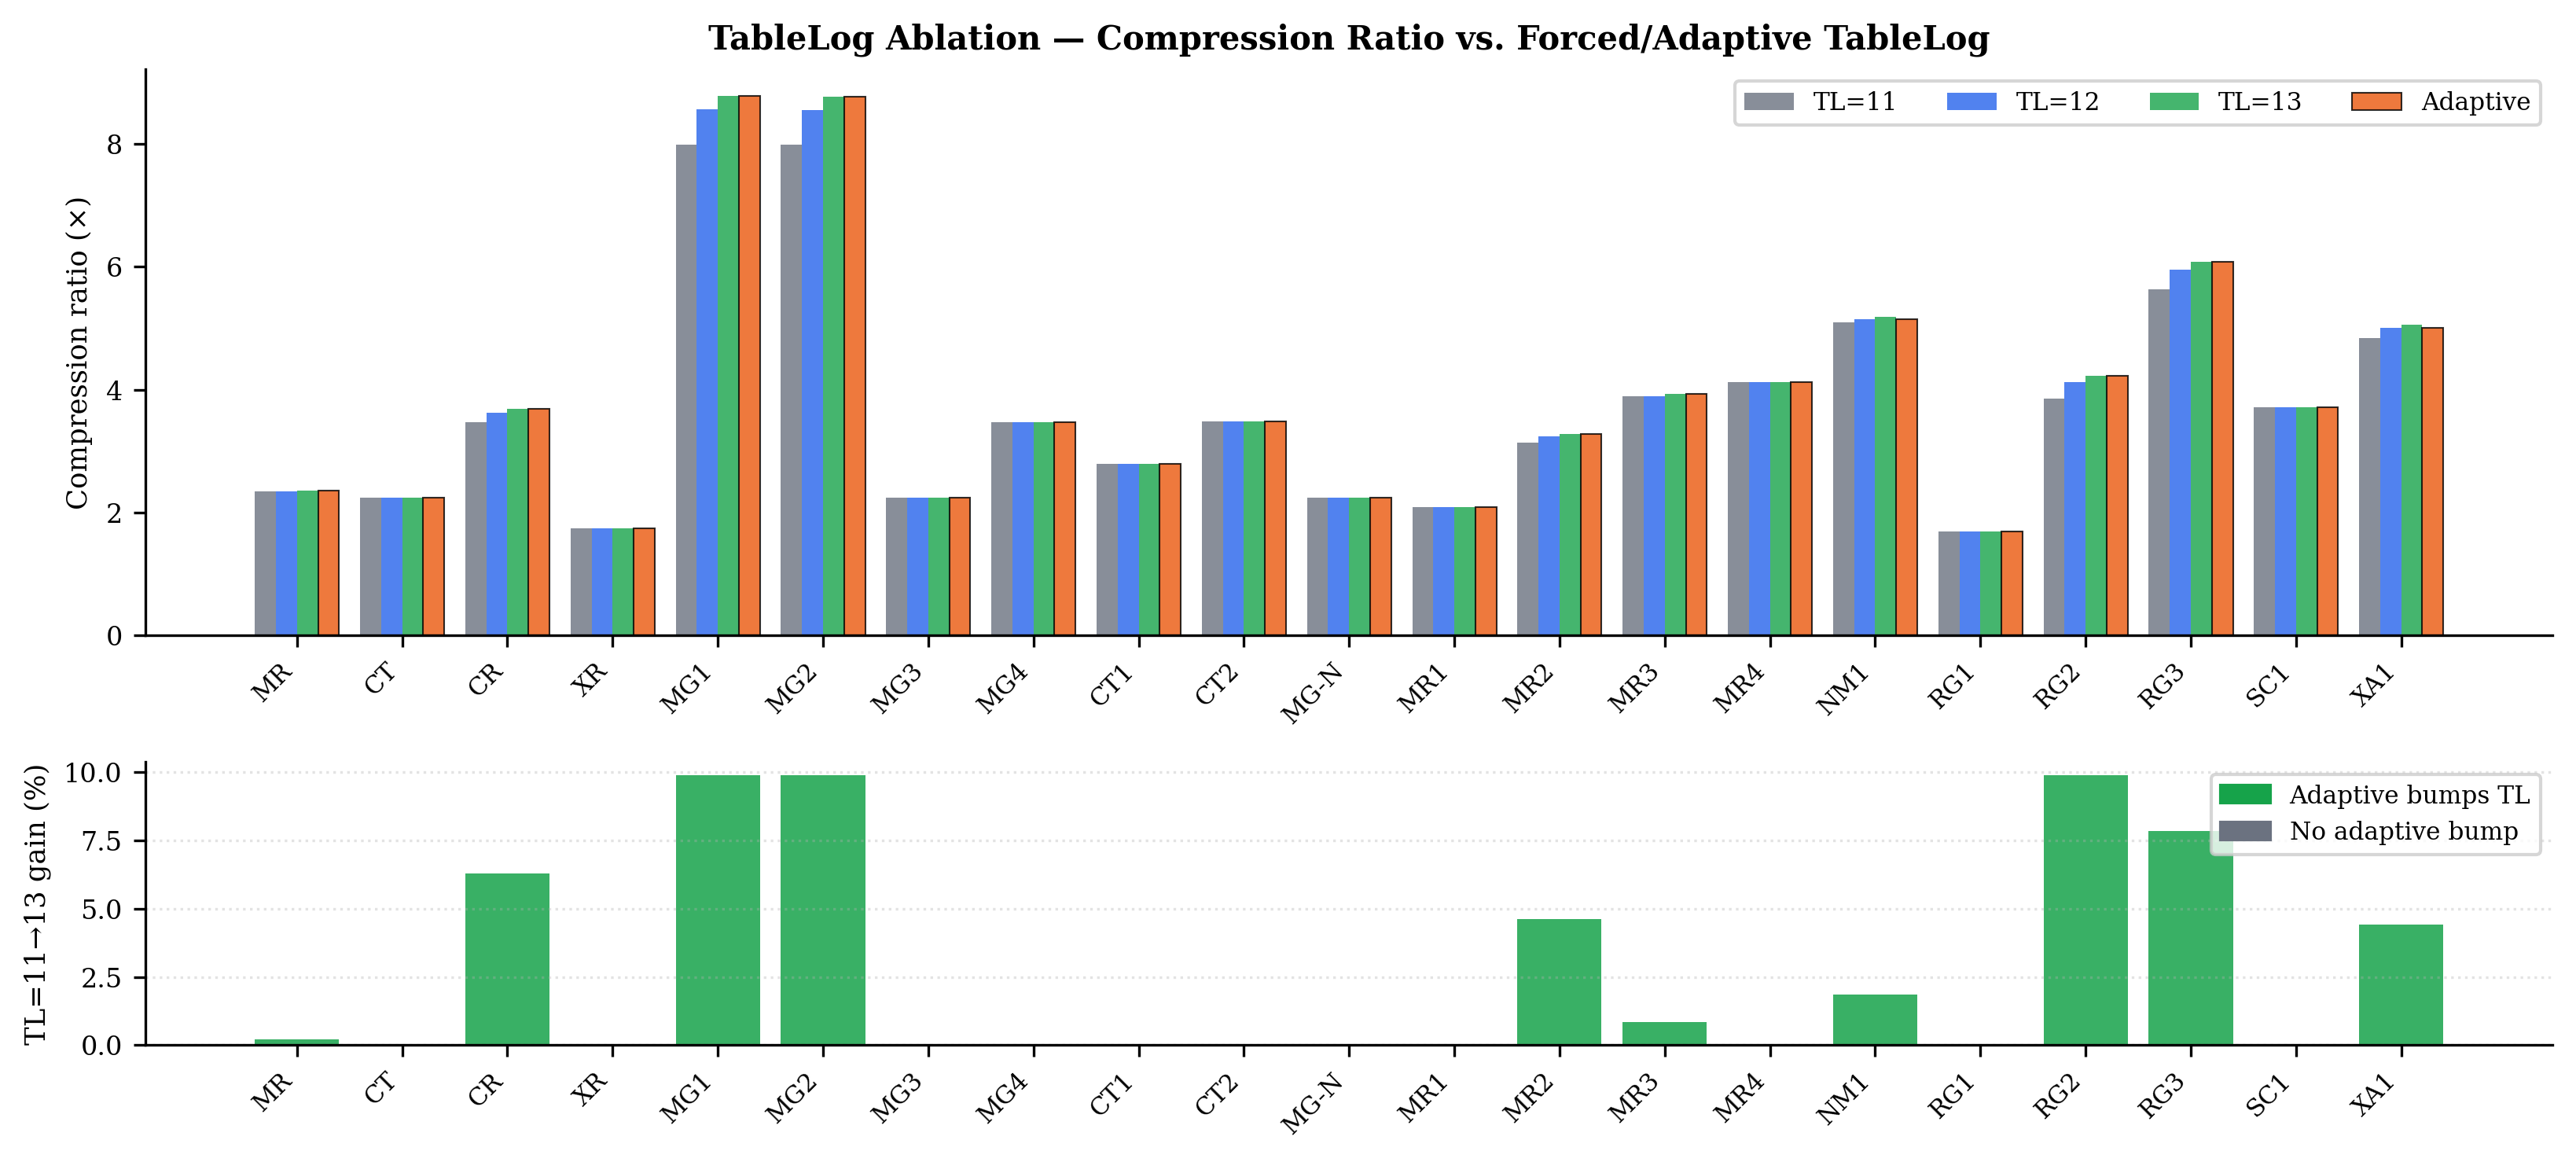
\includegraphics[width=0.85\textwidth]{figures/fig6_tablelog_ablation.png}
\caption{TableLog ablation across all 21 images. Top: absolute compression
ratios for TL=11/12/13 and adaptive selection. Bottom: gain from TL=11$\to$13.}
\label{fig:tablelog-ablation}
\end{figure*}

\subsection{Optional Canonical Huffman Backend}

An optional canonical Huffman backend was implemented for comparison. It
typically produces 1--3\% smaller output than FSE but decodes more slowly due to
variable-length code lookup. Since this paper focuses on the ratio-throughput
tradeoff, FSE is used as the primary backend.

\subsection{RGB and Multi-Frame Extensions}

MIC includes:
\begin{itemize}
  \item \textbf{MIC2} for multi-frame grayscale data with two modes: independent
  (per-frame spatial Delta+RLE+FSE) and temporal (inter-frame ZigZag-encoded
  residuals).
  \item \textbf{MICR} for single-frame RGB images using a reversible YCoCg-R
  transform~\cite{ycocgr} followed by per-plane Delta+RLE+FSE applied to the
  full image without tiling.
\end{itemize}

These modes are included to demonstrate extensibility; the main contribution
remains the grayscale 16-bit lossless pipeline.

% ============================================================
\section{Multi-State Entropy Decoding}
\label{sec:multistate}

\subsection{The Serial Dependency Problem}

A conventional single-state table-based ANS decoder contains a serial
dependency chain:
\begin{equation}
\begin{aligned}
  \text{let } e &= \texttt{decTable}[s_n], \\
  s_{n+1} &= e.\textit{newState} + \texttt{getBits}(e.\textit{nbBits}).
\end{aligned}
\end{equation}
With a table-lookup latency of approximately $L \approx 4$ cycles on modern
out-of-order CPUs (L1 cache hit), the loop is limited to roughly one symbol per
$L$ cycles regardless of available execution units. Modern CPUs have 4--6
execution ports; a single-state ANS decoder uses exactly one dependency chain,
leaving 75--83\% of the hardware capacity idle.

\subsection{Interleaved Decoding}

MIC breaks this dependency by running multiple independent state machines on
interleaved symbol positions. In the four-state design, four independent chains
(A, B, C, D) reconstruct positions:
\begin{align*}
  \text{chain A}&: 0, 4, 8, \ldots \\
  \text{chain B}&: 1, 5, 9, \ldots \\
  \text{chain C}&: 2, 6, 10, \ldots \\
  \text{chain D}&: 3, 7, 11, \ldots
\end{align*}

The four chains are completely independent: each has its own state variable, its
own sequence of table lookups, and its own bit-extraction operations. The CPU's
out-of-order engine sees four simultaneous table-lookup address streams.

\textbf{Latency model.} Let $L$ be the table-lookup latency (cycles).
Single-state FSE processes 1 symbol per $L$ cycles. The $k$-state decoder
processes $k$ symbols per $L$ cycles (amortized):

\begin{table}[htbp]
\centering
\caption{Multi-state decoder latency model and empirical speedup.}
\label{tab:latency}
\begin{tabular}{clrr}
\toprule
States ($k$) & Amortized latency & Theoretical & Empirical \\
\midrule
1 & $L$ cy/sym & 1.0$\times$ & 1.0$\times$ \\
2 & $L/2$ cy/sym & 2.0$\times$ & 1.3$\times$ \\
4 & $L/4$ cy/sym & 4.0$\times$ & 2.0$\times$ \\
\bottomrule
\end{tabular}
\end{table}

The empirical speedup is below theoretical maximum due to: (1) bit-reader
refill overhead shared across all chains, (2) instruction cache pressure from
the unrolled loop, and (3) memory bandwidth limits on compressed stream reads.

\subsection{Correctness}

Correctness follows from partitioning the output sequence into independent
subsequences during encoding and reversing that assignment during decoding.
Each chain operates on a strict subset of positions with no data dependency on
other chains; correctness follows from the correctness of single-state FSE
applied independently to each subset.

\subsection{Stream Signaling}

The bitstream includes a small mode signal: magic sequence \texttt{0xFF,
0x02} for two-state; \texttt{0xFF, 0x04} for four-state; followed by a 4-byte
symbol count. The magic byte \texttt{0xFF} cannot appear as a valid single-state
FSE header (it would imply $\textit{tableLog} = 20$, which exceeds
$\textit{tableLogAbsoluteMax} = 17$), so all three formats coexist without
ambiguity.

\subsection{Platform-Specific Kernels}

\textbf{AMD64 (BMI2):} Uses \texttt{SHLXQ}/\texttt{SHRXQ} for 3-operand
variable shifts, enabling four independent bit-extraction sequences per
iteration without CL register contention. Also includes an interleaved
histogram routine using 4-way unrolled loops.

\textbf{ARM64:} Uses \texttt{LSLV}/\texttt{LSRV} variable-shift instructions
which natively take the count from any general-purpose register.

\textbf{Fallback:} Pure-Go implementations of all routines provide identical
functionality on all non-AMD64/ARM64 targets.

\subsection{Isolated FSE Decompression Throughput}

Table~\ref{tab:fse-arm64} presents isolated FSE decompression throughput for
all 21 images on Apple M2 Max (ARM64, pure Go).

\begin{table}[htbp]
\centering
\caption{Isolated FSE decompression throughput (MB/s), Apple M2 Max (ARM64,
pure Go). MB/s over uncompressed RLE symbol stream.}
\label{tab:fse-arm64}
\scriptsize
\begin{tabular}{lrrrr}
\toprule
Image & 1-state & 2-state & 4-state & 4 vs.\ 1 \\
\midrule
MR   &   514 &   689 &   841 & $+$64\% \\
CT   &   829 &   995 & 1,295 & $+$56\% \\
CR   &   140 & 1,044 &   966 & $+$590\%$^*$ \\
XR   & 1,444 & 1,774 & 1,952 & $+$35\% \\
MG1  & 1,140 & 1,746 & 1,873 & $+$64\% \\
MG2  &   743 & 1,064 & 1,319 & $+$77\% \\
MG3  & 1,453 & 4,115 & 5,462 & $+$276\% \\
MG4  & 2,633 & 3,707 & 5,287 & $+$101\% \\
CT1  &   982 & 1,241 & 1,572 & $+$60\% \\
CT2  & 1,108 & 1,092 & 1,434 & $+$29\% \\
MG-N & 2,944 & 4,138 & 5,696 & $+$94\% \\
MR1  & 1,562 & 2,027 & 2,591 & $+$66\% \\
MR2  & 2,306 & 2,867 & 3,521 & $+$53\% \\
MR3  & 1,472 & 1,582 & 1,841 & $+$25\% \\
MR4  & 1,779 & 1,973 & 2,389 & $+$34\% \\
NM1  & 1,658 & 1,898 & 2,254 & $+$36\% \\
RG1  & 1,676 & 2,652 & 3,128 & $+$87\% \\
RG2  & 2,432 & 3,409 & 3,810 & $+$57\% \\
RG3  & 2,143 & 2,995 & 3,587 & $+$67\% \\
SC1  & 1,997 & 2,788 & 2,927 & $+$47\% \\
XA1  & 2,005 & 2,348 & 2,639 & $+$32\% \\
\midrule
\textbf{Geomean} & \textbf{1,418} & \textbf{1,945} & \textbf{2,375} & \textbf{$+$68\%} \\
\bottomrule
\end{tabular}
\end{table}

$^*$\textbf{CR anomaly}: The single-state CR result (140~MB/s) is caused by the
\texttt{zeroBits} flag: when any symbol probability exceeds 50\%, the
single-state decoder must bounds-check every \texttt{getBits} call. Multi-state
decoders interleave their bit reads, reducing the frequency of this check.

\begin{figure*}[tbp]
\centering
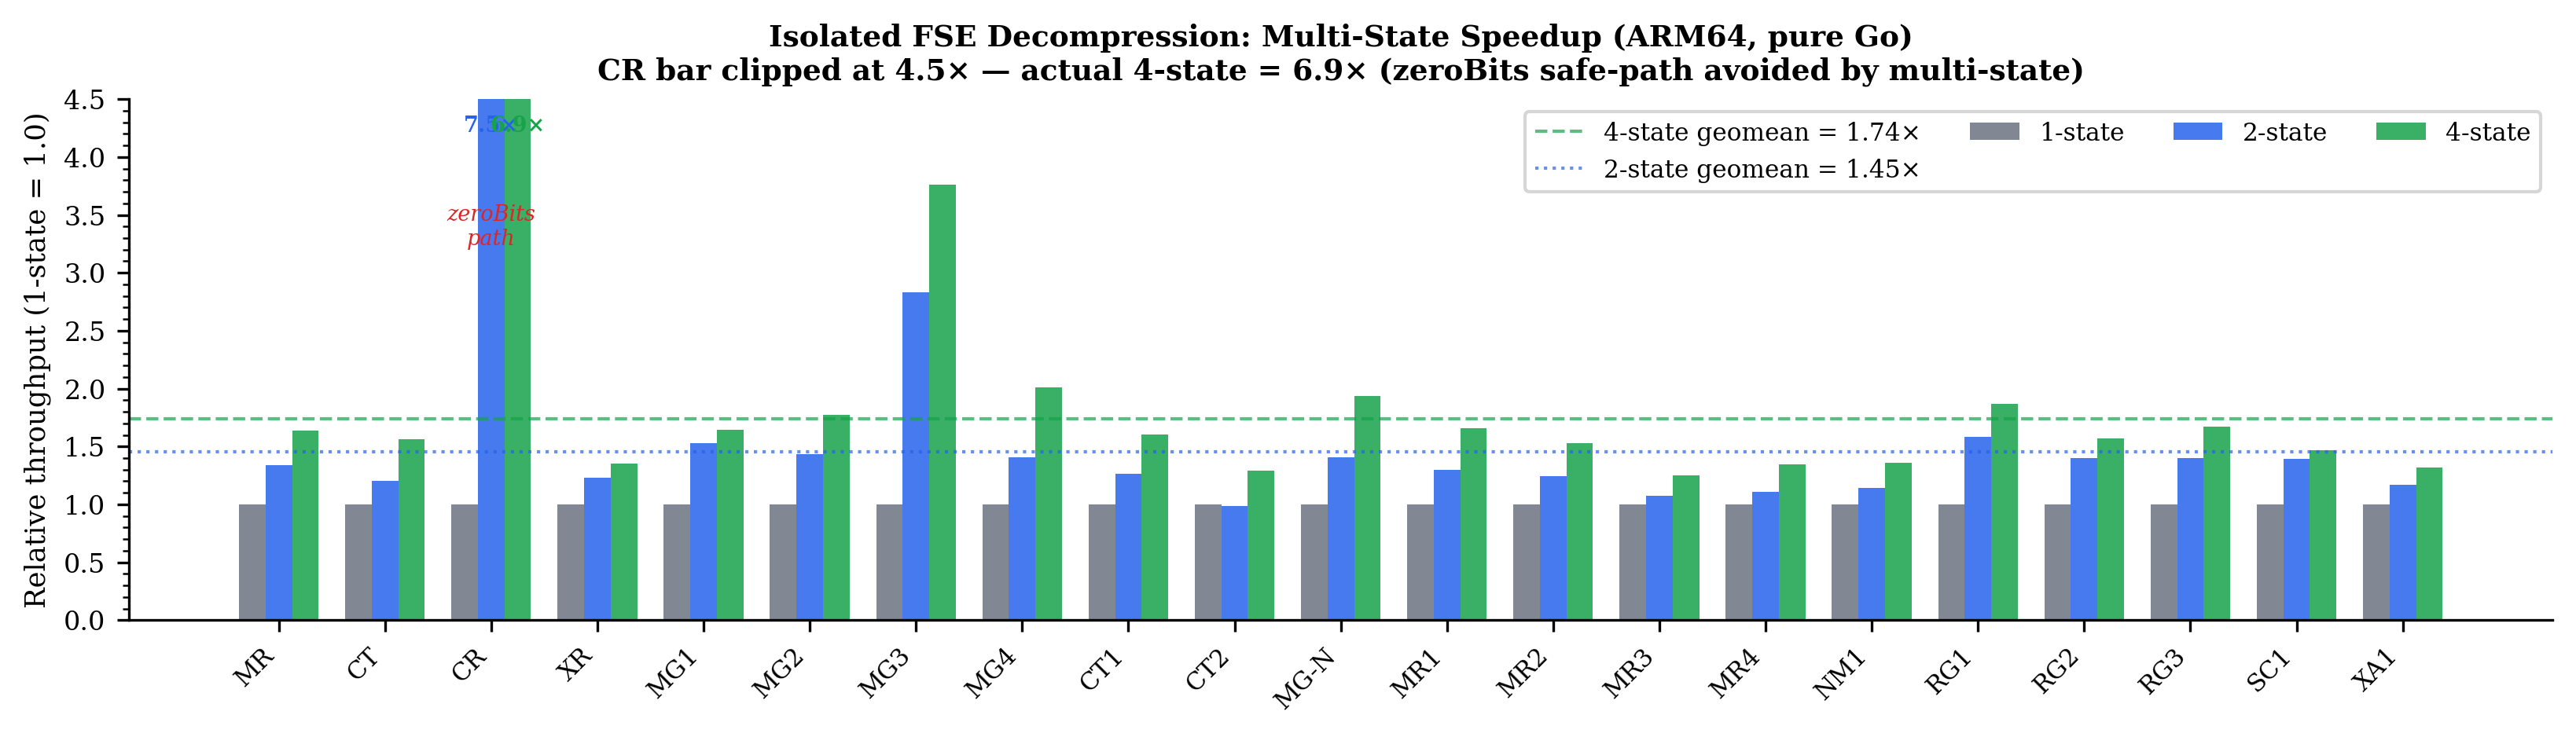
\includegraphics[width=0.85\textwidth]{figures/fig3_multistate_speedup.png}
\caption{Isolated FSE decompression speedup relative to 1-state for all 21
images (ARM64, pure Go). Dashed lines show geomeans: 4-state = 1.74$\times$,
2-state = 1.45$\times$.}
\label{fig:multistate-speedup}
\end{figure*}

Across the 21-image ARM64 sweep in Table~\ref{tab:fse-arm64}, the 4-state
decoder delivers a geometric-mean speedup of $+$68\% over the 1-state
baseline, with per-image gains ranging from $+$25\% (MR3) to $+$590\% (CR,
driven by the \texttt{zeroBits} fast-path discussed above). The spread
reflects how different residual distributions exercise the shared bit-reader
refill path: images with denser symbol alphabets (larger MG, CR) gain the
most, while very small images (MR, NM1) see the least amortization.

Table~\ref{tab:fse-amd64} reports end-to-end MIC decompression throughput on
the Intel Core Ultra 9 285K used for the AMD64 benchmarks in
Section~\ref{sec:methodology}, comparing the pure-Go single-state baseline
(MIC-Go) with the pure-Go four-state interleaved decoder (MIC-4state), across
all 21 images. A 2-state column is omitted because it was not separately
measured on this machine; the values are taken from the
\texttt{BenchmarkAllCodecs} sweep used for Table~\ref{tab:decomp-amd64}. The
4-state decoder delivers a consistent per-image speedup, matching the
qualitative pattern observed on ARM64.

\begin{table}[tbp]
\centering
\caption{Pure-Go MIC decompression throughput (MB/s), Intel Core Ultra 9
285K (AMD64, 24 P-cores), from \texttt{BenchmarkAllCodecs}. MIC-Go is the
single-state FSE decoder; MIC-4state is the four-state interleaved decoder.}
\label{tab:fse-amd64}
\scriptsize
\begin{tabular}{lrrr}
\toprule
Image & MIC-Go (1-state) & MIC-4state & 4 vs.\ 1 \\
\midrule
MR   & 251 & 260 & $+$4\%  \\
CT   & 231 & 243 & $+$5\%  \\
CR   & 324 & 381 & $+$18\% \\
XR   & 363 & 375 & $+$3\%  \\
MG1  & 617 & 630 & $+$2\%  \\
MG2  & 562 & 598 & $+$6\%  \\
MG3  & 357 & 400 & $+$12\% \\
MG4  & 523 & 559 & $+$7\%  \\
CT1  & 322 & 293 & $-$9\%  \\
CT2  & 293 & 295 & $+$1\%  \\
MG-N & 368 & 416 & $+$13\% \\
MR1  & 356 & 351 & $-$1\%  \\
MR2  & 352 & 409 & $+$16\% \\
MR3  & 450 & 443 & $-$2\%  \\
MR4  & 390 & 339 & $-$13\% \\
NM1  & 367 & 339 & $-$8\%  \\
RG1  & 302 & 344 & $+$14\% \\
RG2  & 433 & 472 & $+$9\%  \\
RG3  & 460 & 464 & $+$1\%  \\
SC1  & 464 & 478 & $+$3\%  \\
XA1  & 413 & 415 & $+$0\%  \\
\bottomrule
\end{tabular}
\end{table}

The end-to-end pure-Go speedup on AMD64 is smaller than the isolated-FSE
ARM64 speedup because the 4-state gain is amortised over delta and RLE
stages that execute at the same cost in both variants; for the full C /
BMI2 multi-state decoder throughput on this platform, see the MIC-4state-C
and MIC-4state-SIMD columns of Table~\ref{tab:decomp-amd64}.

% ============================================================
\section{Experimental Methodology}
\label{sec:methodology}

\subsection{Dataset}

The evaluation uses 21 de-identified DICOM images spanning 10 modalities, drawn
from publicly available datasets: NEMA WG-04 compsamples, NEMA 1997 CD, and the
Clunie Breast Tomosynthesis Case~1. All images are de-identified per DICOM PS
3.15 Appendix~E; no ethics approval is required.

\begin{table}[htbp]
\centering
\caption{Test dataset---21 clinical DICOM images spanning 10 modalities.}
\label{tab:dataset}
\scriptsize
\begin{tabular}{llrr}
\toprule
Image & Modality & Dimensions & Raw (MB) \\
\midrule
MR   & Brain MRI      & $256{\times}256$   & 0.13 \\
CT   & CT scan        & $512{\times}512$   & 0.50 \\
CR   & Comp.\ radiography & $2140{\times}1760$ & 7.18 \\
XR   & X-ray          & $2048{\times}2577$ & 10.1 \\
MG1  & Mammography    & $2457{\times}1996$ & 9.35 \\
MG2  & Mammography    & $2457{\times}1996$ & 9.35 \\
MG3  & Mammography    & $4774{\times}3064$ & 27.3 \\
MG4  & Mammography    & $4096{\times}3328$ & 26.0 \\
CT1  & CT scan        & $512{\times}512$   & 0.50 \\
CT2  & CT scan        & $512{\times}512$   & 0.50 \\
MG-N & Mammography    & $3064{\times}4664$ & 27.3 \\
MR1  & Brain MRI      & $512{\times}512$   & 0.50 \\
MR2  & Brain MRI      & $1024{\times}1024$ & 2.00 \\
MR3  & Brain MRI      & $512{\times}512$   & 0.50 \\
MR4  & Brain MRI      & $512{\times}512$   & 0.50 \\
NM1  & Nuclear med.   & $256{\times}1024$  & 0.50 \\
RG1  & Radiography    & $1841{\times}1955$ & 6.86 \\
RG2  & Radiography    & $1760{\times}2140$ & 7.18 \\
RG3  & Radiography    & $1760{\times}1760$ & 5.91 \\
SC1  & Sec.~capture   & $2048{\times}2487$ & 9.71 \\
XA1  & Fluoroscopy    & $1024{\times}1024$ & 2.00 \\
\bottomrule
\end{tabular}
\end{table}

This dataset spans multiple modalities and image sizes but remains modest for
strong generalization claims.

\subsection{Baselines}

The current study compares MIC with:
\begin{itemize}
  \item \textbf{HTJ2K} (OpenJPH~\cite{openjph}), via in-process CGO bindings,
  \item \textbf{JPEG-LS} (CharLS~\cite{charls}), via in-process CGO bindings,
  and
  \item \textbf{Delta\,+\,Zstandard} (level 19).
\end{itemize}

\subsection{Metrics}

The paper reports:
\begin{itemize}
  \item \textbf{Compression ratio}: uncompressed size / compressed size.
  \item \textbf{Decompression throughput}: uncompressed pixel bytes
  reconstructed per second (MB/s).
  \item \textbf{Encoding throughput}: uncompressed pixel bytes processed per
  second (MB/s).
\end{itemize}

\subsection{Benchmark Procedure}

All codecs were measured using in-process library calls on the same machine to
avoid file-I/O and subprocess overhead. The Go testing framework's
\texttt{-benchtime=10x} flag was used.

\textbf{Platforms:}
\begin{itemize}
  \item Apple M2 Max (12-core ARM64), Go compiler with \texttt{-O3}.
  \item Intel Core Ultra 9 285K (24 P-core AMD64),
  \texttt{-O3 -march=native}.
\end{itemize}

\textbf{Variant nomenclature:}
\begin{itemize}
  \item \textbf{MIC-Go}: Pure Go, single-state FSE.
  \item \textbf{MIC-4state}: Pure Go, four-state FSE.
  \item \textbf{MIC-4state-C}: C four-state FSE decoder via CGO.
  \item \textbf{MIC-4state-SIMD}: C four-state FSE with BMI2 (AMD64) or scalar
  (ARM64) via CGO.
  \item \textbf{Wavelet+SIMD}: 5/3 wavelet with blocked column layout + AVX2
  (AMD64) or scalar blocked (ARM64).
  \item \textbf{PICS-C-N}: Parallel Image Compressed Strips with $N$ strips.
\end{itemize}

Run-to-run variance is $<$2\% on Apple M2 Max and $<$5\% on Intel AMD64.

\subsection{JavaScript and Browser Evaluation}

A pure JavaScript decoder (${\sim}$20\,KB ES module, zero npm dependencies) and
a Go WebAssembly build (${\sim}$2.5\,MB) were implemented. Performance
measurements reported in Section~\ref{sec:results} were obtained in Node.js
v24.8 (Apple M2 Max).

% ============================================================
\section{Results}
\label{sec:results}

\subsection{Compression Ratio}

Table~\ref{tab:ratios} presents lossless compression ratios for all codec
variants across the 21-image dataset.

\begin{table*}[t]
\centering
\caption{Lossless compression ratios---all codec variants, 21 images. Bold =
best ratio per row. JPEG-LS consistently achieves the highest ratios.}
\label{tab:ratios}
\scriptsize
\begin{tabular}{lrrrrrrrr}
\toprule
Image & Raw (MB) & $\Delta$+Zstd-19 & MIC & Wavelet & PICS-4 & PICS-8 & HTJ2K & JPEG-LS \\
\midrule
MR   & 0.13 & 1.95$\times$ & 2.35$\times$ & 2.38$\times$ & 2.28$\times$ & 2.21$\times$ & 2.38$\times$ & \textbf{2.52$\times$} \\
CT   & 0.50 & 2.05$\times$ & 2.24$\times$ & 1.67$\times$ & 2.15$\times$ & 1.96$\times$ & 1.77$\times$ & \textbf{2.68$\times$} \\
CR   & 7.18 & 3.24$\times$ & 3.69$\times$ & 3.81$\times$ & 3.70$\times$ & 3.71$\times$ & 3.77$\times$ & \textbf{3.96$\times$} \\
XR   & 10.1 & 1.43$\times$ & 1.74$\times$ & \textbf{1.76$\times$} & 1.75$\times$ & \textbf{1.76$\times$} & 1.67$\times$ & \textbf{1.76$\times$} \\
MG1  & 9.35 & 7.20$\times$ & 8.79$\times$ & 8.67$\times$ & 8.84$\times$ & 8.87$\times$ & 8.25$\times$ & \textbf{8.91$\times$} \\
MG2  & 9.35 & 7.21$\times$ & 8.77$\times$ & 8.65$\times$ & 8.83$\times$ & 8.85$\times$ & 8.24$\times$ & \textbf{8.90$\times$} \\
MG3  & 27.3 & 2.04$\times$ & 2.24$\times$ & 2.32$\times$ & 2.31$\times$ & 2.34$\times$ & 2.22$\times$ & \textbf{2.38$\times$} \\
MG4  & 26.0 & 3.10$\times$ & 3.47$\times$ & 3.59$\times$ & 3.59$\times$ & 3.62$\times$ & 3.51$\times$ & \textbf{3.71$\times$} \\
CT1  & 0.50 & 2.47$\times$ & 2.79$\times$ & 2.49$\times$ & 2.54$\times$ & 2.29$\times$ & 2.70$\times$ & \textbf{3.19$\times$} \\
CT2  & 0.50 & 3.24$\times$ & 3.49$\times$ & 2.87$\times$ & 3.11$\times$ & 2.72$\times$ & 3.29$\times$ & \textbf{4.54$\times$} \\
MG-N & 27.3 & 2.04$\times$ & 2.24$\times$ & 2.32$\times$ & 2.31$\times$ & 2.34$\times$ & 2.23$\times$ & \textbf{2.38$\times$} \\
MR1  & 0.50 & 1.79$\times$ & 2.09$\times$ & 2.14$\times$ & 2.10$\times$ & 2.08$\times$ & 2.13$\times$ & \textbf{2.30$\times$} \\
MR2  & 2.00 & 2.77$\times$ & 3.28$\times$ & 3.34$\times$ & 3.31$\times$ & 3.31$\times$ & 3.35$\times$ & \textbf{3.52$\times$} \\
MR3  & 0.50 & 3.47$\times$ & 3.93$\times$ & 4.09$\times$ & 3.89$\times$ & 3.84$\times$ & 4.33$\times$ & \textbf{4.51$\times$} \\
MR4  & 0.50 & 3.58$\times$ & 4.12$\times$ & 4.18$\times$ & 4.09$\times$ & 4.03$\times$ & 4.21$\times$ & \textbf{4.49$\times$} \\
NM1  & 0.50 & 4.88$\times$ & 5.15$\times$ & 5.02$\times$ & 5.26$\times$ & 5.28$\times$ & 5.76$\times$ & \textbf{6.28$\times$} \\
RG1  & 6.86 & 1.45$\times$ & 1.70$\times$ & 1.70$\times$ & 1.70$\times$ & 1.69$\times$ & 1.63$\times$ & \textbf{1.72$\times$} \\
RG2  & 7.18 & 3.68$\times$ & 4.23$\times$ & 4.32$\times$ & 4.28$\times$ & 4.30$\times$ & 4.32$\times$ & \textbf{4.51$\times$} \\
RG3  & 5.91 & 5.46$\times$ & 6.08$\times$ & 6.82$\times$ & 6.11$\times$ & 6.12$\times$ & 6.99$\times$ & \textbf{7.31$\times$} \\
SC1  & 9.71 & 3.46$\times$ & 3.71$\times$ & 3.70$\times$ & 3.73$\times$ & 3.74$\times$ & 3.85$\times$ & \textbf{4.73$\times$} \\
XA1  & 2.00 & 4.37$\times$ & 5.01$\times$ & 4.94$\times$ & 5.04$\times$ & 5.03$\times$ & 4.88$\times$ & \textbf{5.39$\times$} \\
\bottomrule
\end{tabular}
\end{table*}

\textbf{Summary statistics:}

\begin{table}[htbp]
\centering
\caption{Compression ratio summary---geometric means and win counts.}
\label{tab:ratio-summary}
\begin{tabular}{lrr}
\toprule
Codec & Geo.\ Mean & Best on \\
\midrule
JPEG-LS & \textbf{3.44$\times$} & 21/21 \\
Wavelet V2 SIMD & 3.28$\times$ & 0/21 \\
HTJ2K & 3.15$\times$ & 0/21 \\
MIC (Delta+RLE+FSE) & 3.12$\times$ & 0/21 \\
Delta+Zstd-19 & 3.03$\times$ & 0/21 \\
\bottomrule
\end{tabular}
\end{table}

\textbf{Analysis.} JPEG-LS achieves the highest lossless ratio on all 21
images. MIC's strength is not in ratio but in the ratio-throughput-simplicity
tradeoff: it achieves 91\% of JPEG-LS's geometric mean ratio at 4$\times$ the
decompression throughput and 1/5 the implementation complexity.

Mammography achieves the highest MIC ratios (up to 8.79$\times$) due to smooth
tissue regions producing near-zero RLE runs. CT with full 16-bit dynamic range
achieves 2.24$\times$ (MIC) vs.\ 1.67$\times$ (Wavelet): coefficient overflow in
the 5/3 lifting step inflates Wavelet compressed size.

\textbf{PICS strip adaptation.} Large images improve compression with more
strips because each strip receives a dedicated FSE table that specializes to its
local residual distribution: $\sum_k |S_k| \cdot H(S_k) < |S| \cdot H(S)$.

\subsection{Effect of 16-Bit-Native Residual Coding}

MIC outperforms Delta+Zstandard (zstd level 19) by 5--22\% on all 21 tested
images (geometric mean $+$14\%). The gap is structural: the mutual information
$I(X_H;\, X_L)$ of delta residuals ranges from 0.3\,bits/symbol (MR) to
1.1\,bits/symbol (MG3), matching the empirical range.

\subsection{Decompression Throughput---ARM64}

Table~\ref{tab:decomp-arm} presents decompression throughput on Apple M2 Max.
MIC-4state-C is the fastest single-threaded decoder on 13/21 images; PICS-C-8
exceeds HTJ2K on all 21 images.

\begin{table*}[t]
\centering
\caption{Decompression throughput (MB/s), Apple M2 Max (ARM64). Bold = fastest
per row (single-threaded: first 5 cols; PICS: last 3 cols).}
\label{tab:decomp-arm}
\scriptsize
\begin{tabular}{lrrrrrrrr}
\toprule
Image & MIC-Go & MIC-4s-C & Wav+SIMD & HTJ2K & JPEG-LS & PICS-C-2 & PICS-C-4 & PICS-C-8 \\
\midrule
MR   & 144 & \textbf{348} & 248 & 265 & 102 & 530 & \textbf{710}$^\dagger$ & 482 \\
CT   & 191 & \textbf{356} & 316 & 307 & 137 & 524 & 955 & \textbf{1,092} \\
CR   & 296 & 524 & \textbf{567} & 367 & 153 & 867 & 1,635 & \textbf{2,661} \\
XR   & 308 & 533 & \textbf{627} & 334 & 108 & 874 & 1,666 & \textbf{3,025} \\
MG1  & 482 & 683 & 678 & \textbf{810} & 409 & 1,205 & 2,112 & \textbf{3,656} \\
MG2  & 479 & 686 & 697 & \textbf{790} & 416 & 1,225 & 2,120 & \textbf{3,773} \\
MG3  & 308 & \textbf{531} & 422 & 338 & 153 & 864 & 1,673 & \textbf{3,117} \\
MG4  & 417 & \textbf{625} & 516 & 548 & 184 & 1,093 & 2,004 & \textbf{3,689} \\
CT1  & 239 & \textbf{436} & 425 & 362 & 182 & 686 & 1,013 & \textbf{1,183} \\
CT2  & 238 & 439 & \textbf{481} & 375 & 175 & 676 & 1,041 & \textbf{1,189} \\
MG-N & 316 & \textbf{536} & 468 & 340 & 153 & 883 & 1,711 & \textbf{3,175} \\
MR1  & 278 & \textbf{521} & 435 & 325 & 116 & 751 & 1,207 & \textbf{1,402} \\
MR2  & 333 & \textbf{563} & 498 & 388 & 172 & 913 & 1,552 & \textbf{2,466} \\
MR3  & 375 & \textbf{639} & 507 & 441 & 236 & 908 & 1,430 & \textbf{1,614} \\
MR4  & 316 & \textbf{571} & 479 & 406 & 197 & 818 & 1,341 & \textbf{1,558} \\
NM1  & 327 & \textbf{632} & 575 & 410 & 210 & 888 & 1,400 & \textbf{1,679} \\
RG1  & 235 & 406 & \textbf{584} & 332 & 104 & 602 & 1,128 & \textbf{2,017} \\
RG2  & 367 & 590 & \textbf{644} & 443 & 193 & 986 & 1,803 & \textbf{3,194} \\
RG3  & 374 & 604 & \textbf{656} & 562 & 246 & 1,035 & 1,944 & \textbf{3,302} \\
SC1  & 375 & \textbf{587} & 388 & 401 & 229 & 1,017 & 1,861 & \textbf{3,279} \\
XA1  & 331 & \textbf{576} & 459 & 419 & 204 & 928 & 1,583 & \textbf{2,493} \\
\bottomrule
\end{tabular}
\end{table*}

$^\dagger$MR is too small for PICS-C-8; PICS-C-4 is best.
MIC-4state-C is 1.7--5.0$\times$ faster than JPEG-LS on all 21 images.
PICS-C-8 peaks at 3,773\,MB/s on MG2.

\subsection{Decompression Throughput---AMD64}

Table~\ref{tab:decomp-amd64} presents results on AMD64 where MIC-4state-SIMD
activates BMI2/PDEP and Wavelet+SIMD gains AVX2 kernels.

\begin{table*}[t]
\centering
\caption{Decompression throughput (MB/s), Intel Core Ultra 9 285K (AMD64).
Bold = fastest per row within single-threaded and PICS groups.}
\label{tab:decomp-amd64}
\scriptsize
\begin{tabular}{lrrrrrrr}
\toprule
Image & MIC-Go & MIC-4s-C & MIC-4s-SIMD & Wav+SIMD & HTJ2K & PICS-C-4 & PICS-C-8 \\
\midrule
MR   & 251 & 501 & \textbf{708} & 194 & 570 & 301 & 124$^\dagger$ \\
CT   & 231 & 403 & 487 & 364 & \textbf{544} & \textbf{676} & 339 \\
CR   & 324 & 599 & \textbf{744} & 723 & 708 & 1,738 & \textbf{2,435} \\
XR   & 363 & 601 & \textbf{803} & 681 & 570 & 1,714 & \textbf{1,994} \\
MG1  & 617 & 789 & 1,119 & 746 & \textbf{1,235} & 1,872 & \textbf{2,514} \\
MG2  & 562 & 800 & 1,166 & 848 & \textbf{1,297} & \textbf{2,244} & 2,085 \\
MG3  & 357 & 633 & 669 & \textbf{678} & 644 & 1,823 & \textbf{2,538} \\
MG4  & 523 & 743 & 773 & \textbf{808} & 916 & 2,124 & \textbf{2,707} \\
CT1  & 322 & 520 & \textbf{676} & 525 & 657 & \textbf{857} & 423 \\
CT2  & 293 & 514 & 636 & \textbf{705} & 627 & \textbf{847} & 687 \\
MG-N & 368 & 635 & 669 & \textbf{705} & 643 & 1,872 & \textbf{2,191} \\
MR1  & 356 & 609 & \textbf{766} & 532 & 654 & \textbf{945} & 366 \\
MR2  & 352 & 658 & \textbf{975} & 601 & 749 & \textbf{1,121} & 793 \\
MR3  & 450 & 728 & \textbf{809} & 676 & 802 & \textbf{920} & 705 \\
MR4  & 390 & 596 & \textbf{861} & 738 & 660 & 493 & \textbf{701} \\
NM1  & 367 & \textbf{717} & 668 & 715 & 627 & \textbf{783} & 405 \\
RG1  & 302 & 497 & 593 & \textbf{705} & 557 & 1,248 & \textbf{1,494} \\
RG2  & 433 & 676 & \textbf{861} & 811 & 823 & 1,841 & \textbf{1,912} \\
RG3  & 460 & 706 & 858 & 881 & \textbf{894} & \textbf{1,969} & 1,613 \\
SC1  & 464 & 695 & \textbf{888} & 710 & 728 & 1,819 & \textbf{1,889} \\
XA1  & 413 & 693 & \textbf{836} & 538 & 797 & 1,173 & \textbf{1,513} \\
\bottomrule
\end{tabular}
\end{table*}

On AMD64, MIC-4state-SIMD leads 16/21 images single-threaded; HTJ2K leads on
MG1, MG2, MG4, CT, and RG3. PICS-C-8 exceeds HTJ2K on all 21 images on both
platforms.

\subsection{Encoding Throughput}

Table~\ref{tab:encoding} summarizes encoding throughput on ARM64.

\begin{table}[htbp]
\centering
\caption{Encoding throughput (MB/s), Apple M2 Max (ARM64), selected images.
Bold = fastest per row.}
\label{tab:encoding}
\scriptsize
\begin{tabular}{lrrrrrr}
\toprule
Image & MIC-Go & MIC-4s-C & MIC-C & HTJ2K & JPEG-LS & PICS-8 \\
\midrule
MR  & 180 & 243 & \textbf{305} & 217 & 104 & 103 \\
CT  & 208 & 314 & 332 & 258 & 166 & \textbf{358} \\
CR  & 307 & 441 & 416 & 311 & 119 & \textbf{1,195} \\
XR  & 336 & 498 & 500 & 269 & 123 & \textbf{1,136} \\
MG1 & 512 & 621 & 651 & 676 & 320 & \textbf{2,001} \\
MG2 & 517 & 644 & 702 & 700 & 315 & \textbf{2,095} \\
MG3 & 355 & 469 & 425 & 293 & 153 & \textbf{1,491} \\
MG4 & 458 & 554 & 503 & 451 & 234 & \textbf{1,984} \\
\bottomrule
\end{tabular}
\end{table}

MIC-4state-C is 2--2.5$\times$ faster than pure-Go MIC-Go on all images.
JPEG-LS is consistently 2--4$\times$ slower to encode than MIC-Go. PICS-8
reaches 1.2--2.1\,GB/s on large images, sufficient for real-time PACS
ingestion.

\subsection{JavaScript Runtime Results}

Table~\ref{tab:js-perf} reports Node.js single-threaded performance;
Table~\ref{tab:pics-js} reports parallel PICS decoding via
\texttt{worker\_threads}.

\begin{table}[htbp]
\centering
\caption{JavaScript decoder throughput (4-state), Node.js v24.8, Apple M2 Max.
Median over 20 iterations.}
\label{tab:js-perf}
\begin{tabular}{lrrrr}
\toprule
Image & Dimensions & Ratio & ms & MB/s \\
\midrule
MR  & $256{\times}256$ & 2.35$\times$ & 3.0 & 42 \\
CT  & $512{\times}512$ & 2.24$\times$ & 13.5 & 37 \\
CR  & $1760{\times}2140$ & 3.69$\times$ & 161.2 & 45 \\
MG1 & $1996{\times}2457$ & 8.79$\times$ & 80.9 & 116 \\
MG3 & $3064{\times}4774$ & 2.29$\times$ & 638.4 & 44 \\
\bottomrule
\end{tabular}
\end{table}

\begin{table}[htbp]
\centering
\caption{PICS parallel JavaScript decoder (\texttt{worker\_threads}), Apple M2
Max. Speedup relative to 1 worker.}
\label{tab:pics-js}
\begin{tabular}{lrrrr}
\toprule
Image & Strips & ms & MB/s & Speedup \\
\midrule
MR  & 4 & 1.3 & 94 & 2.57$\times$ \\
CT  & 4 & 5.0 & 101 & 2.95$\times$ \\
CR  & 8 & 31.7 & 227 & 5.53$\times$ \\
MG1 & 8 & 19.4 & 483 & 4.36$\times$ \\
\bottomrule
\end{tabular}
\end{table}

MG1 (9.35\,MB) decompresses in 19.4\,ms at 483\,MB/s using 12 workers. A
web-based DICOM viewer can fetch a \texttt{.mic} file directly from object
storage and decode it client-side---zero server-side compute, zero transcoding
latency.

\textbf{Limitation.} Node.js \texttt{worker\_threads} performance is not
equivalent to browser Web Worker performance. Full browser performance remains
to be validated.

% ============================================================
\section{Discussion}
\label{sec:discussion}

\subsection{Why a Simple Residual Pipeline Can Be Effective}

A practical conclusion from the current study is that simple prediction can
already remove much of the redundancy in many medical images. When the residual
stream becomes concentrated near zero and repeated values are common, a direct
residual-domain representation can be highly effective.

Fig.~\ref{fig:histogram} shows the empirical delta-residual distributions for
five representative modalities after the avg spatial predictor. All five are
sharply concentrated near zero, with MG1 (mammography) placing 69.2\% of all
residuals at exactly zero---explaining its exceptional compression ratio
(8.79$\times$).

\begin{figure*}[tbp]
\centering
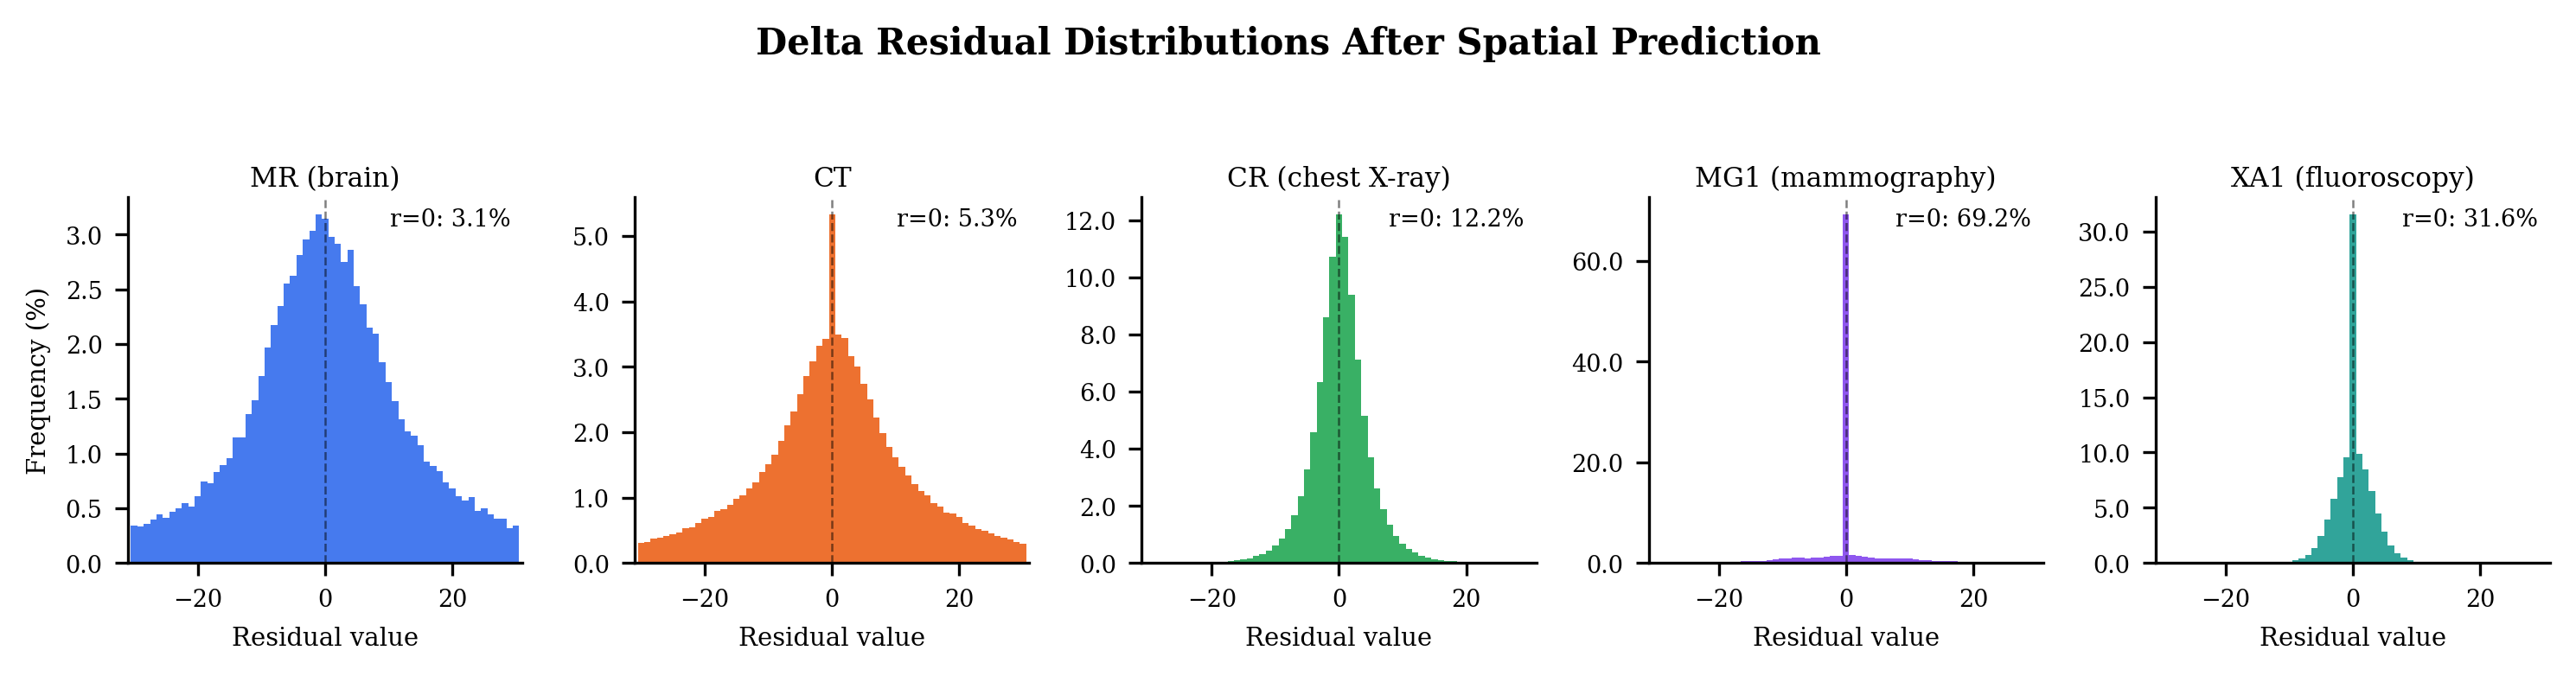
\includegraphics[width=0.85\textwidth]{figures/fig2_histogram.png}
\caption{Delta-residual distributions ($|r| \leq 30$ shown) after avg spatial
prediction. MG1's extreme concentration (69.2\% at zero) explains its
8.79$\times$ compression ratio.}
\label{fig:histogram}
\end{figure*}

\subsection{The Cost-of-Complexity Frontier}

Table~\ref{tab:pareto} places MIC against the main reference codecs on three
axes: compression ratio (geometric mean over the 21 images), decompression
throughput, and decoder source size. JPEG-LS wins on ratio but is the
slowest to decode; HTJ2K is ratio-competitive but ships as
${\sim}$20k lines of C++ with no browser decoder. MIC's core Delta+RLE+FSE
pipeline sits close to both on ratio while decoding faster than JPEG-LS and
fitting in roughly 1k lines---small enough to ship as a zero-dependency
JavaScript module.

\begin{table}[tbp]
\centering
\caption{Ratio vs.\ decompression throughput (geometric means) and decoder
source size.}
\label{tab:pareto}
\scriptsize
\begin{tabular}{lrrrp{1.2cm}}
\toprule
Codec & Ratio & Decomp. & LOC & Browser \\
\midrule
$\Delta$+RLE+FSE (Go) & 3.12$\times$ & 310 & 1.1k & \textbf{Yes} \\
$\Delta$+RLE+FSE (4s-C) & 3.12$\times$ & 530 & 1.5k & \textbf{Yes} \\
HTJ2K (OpenJPH) & 3.15$\times$ & 460 & 20k & No \\
JPEG-LS (CharLS) & 3.44$\times$ & 130 & 5.0k & No \\
\bottomrule
\end{tabular}
\end{table}

\begin{figure*}[tbp]
\centering
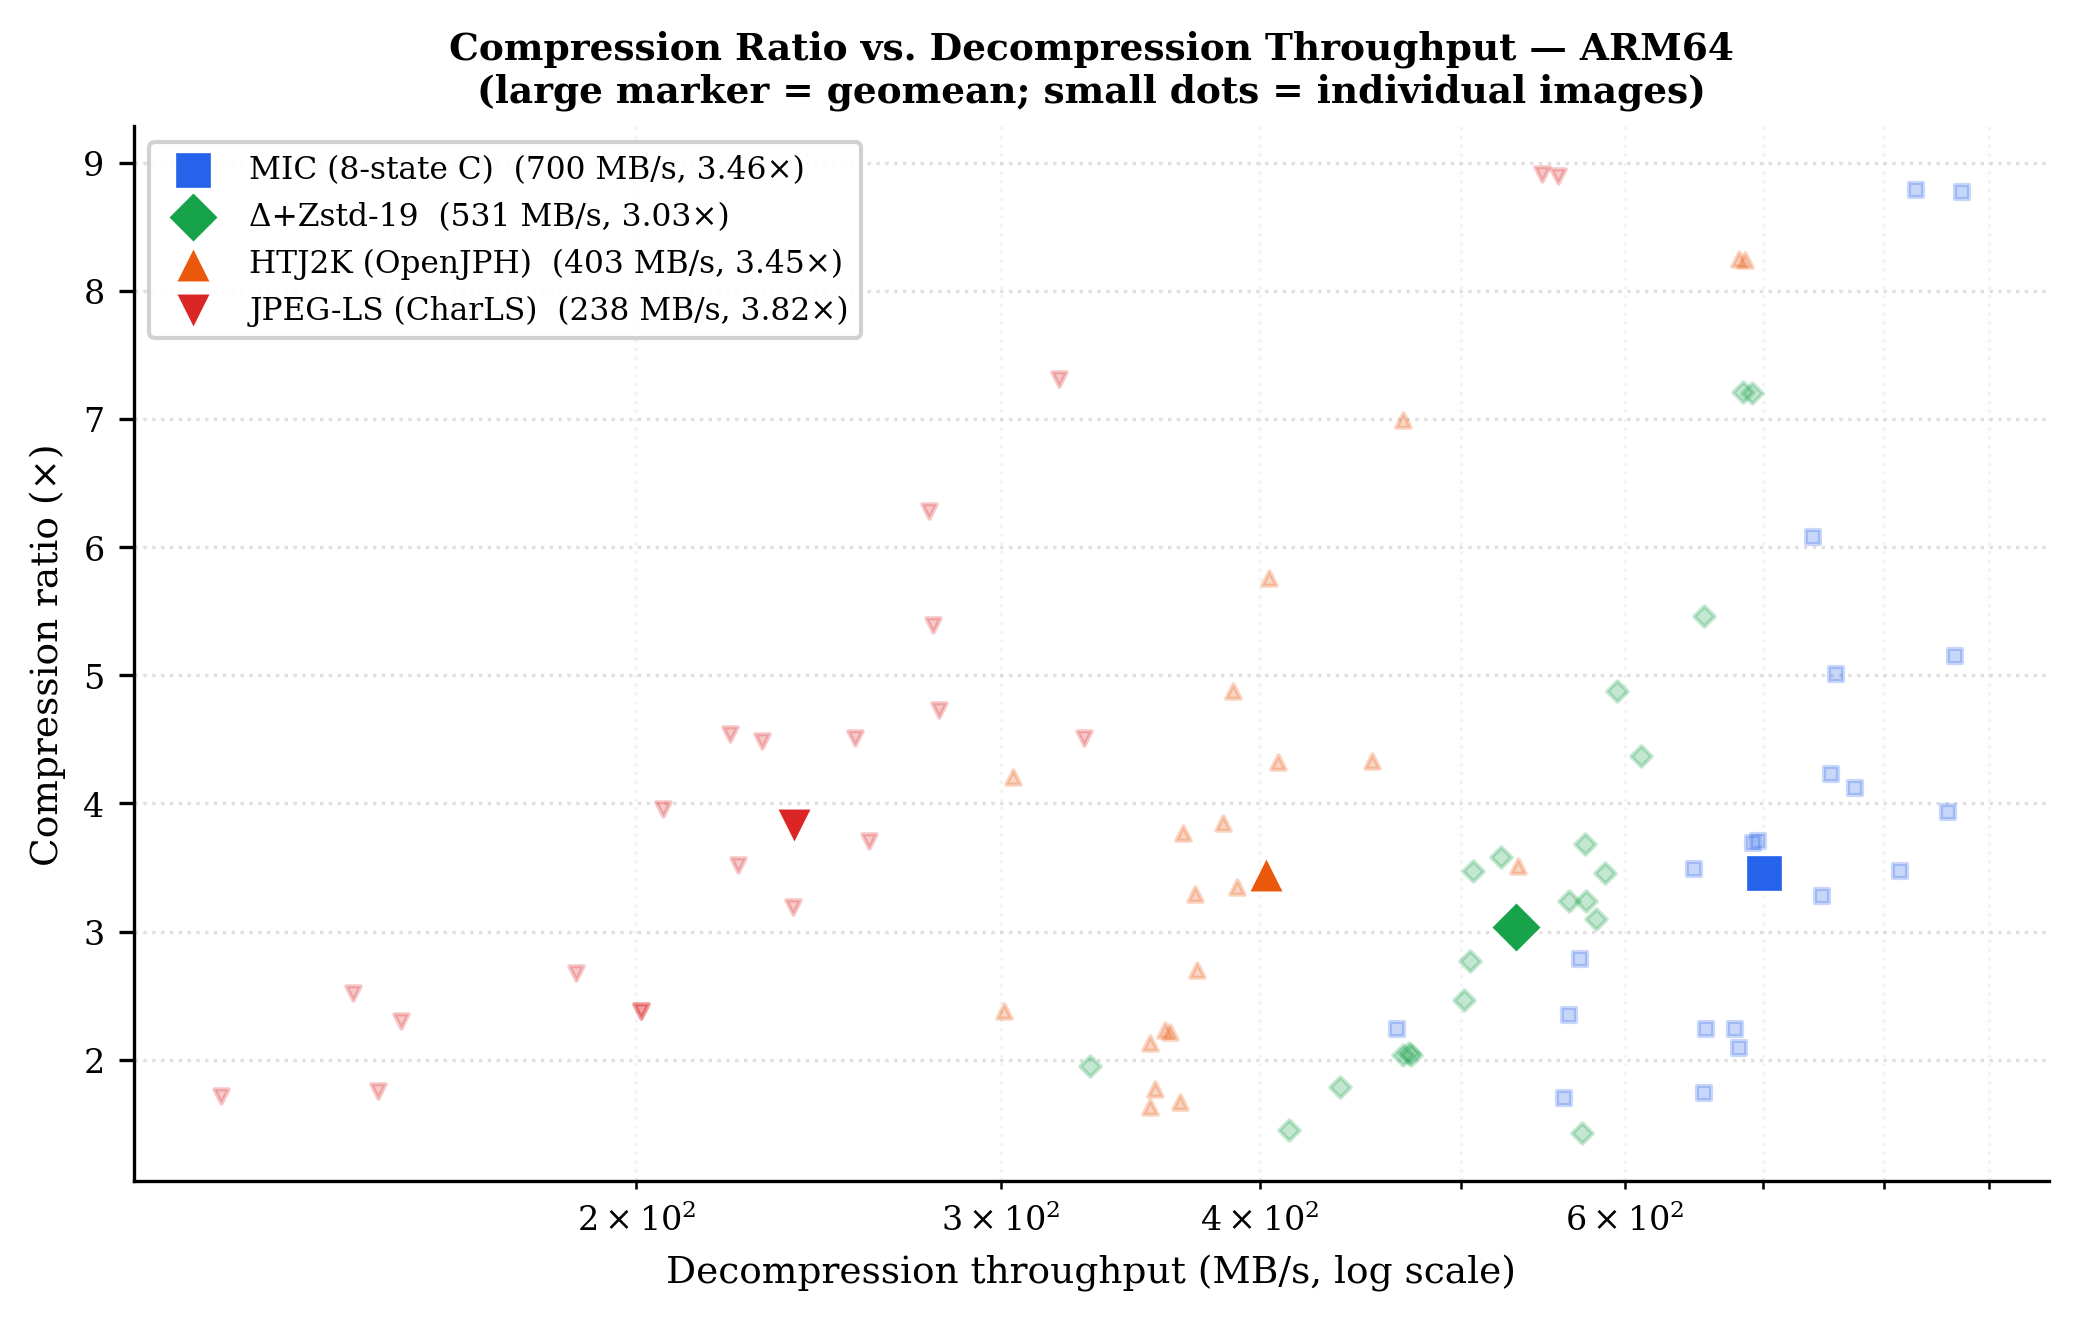
\includegraphics[width=0.85\textwidth]{figures/fig4_pareto.png}
\caption{Compression ratio vs.\ decompression throughput (ARM64). Large
markers = geometric means; small dots = individual images.}
\label{fig:pareto}
\end{figure*}

\subsection{Lightweight Client-Side Decoding}

MIC ships two browser decoder implementations: a pure JS ES module
(${\sim}$20\,KB, zero dependencies) and a Go WASM build (${\sim}$2.5\,MB). A
web-based DICOM viewer can fetch a \texttt{.mic} file directly from object
storage and decode it client-side, eliminating server-side transcoding. As of
the submission date, no production-ready WebAssembly or JavaScript decoder exists
for HTJ2K~\cite{nohtj2k} or JPEG-LS~\cite{charls}.

\subsection{Pathway to Clinical Impact}

MIC could be registered as a DICOM Private Transfer Syntax, allowing PACS
vendors to adopt it without modifying the DICOM standard. The ${\sim}$20\,KB
JavaScript decoder enables a direct storage-and-serve distribution model that
bypasses server-side transcoding entirely.

% ============================================================
\section{Conclusion}
\label{sec:conclusion}

This paper presented MIC, a lossless medical image compression pipeline based on
spatial prediction, 16-bit-native run-length representation, and large-alphabet
table-based entropy coding. The key results across 21 clinical DICOM images
spanning 10 modalities:

\begin{itemize}
  \item \textbf{Compression ratios}: 1.7$\times$--8.9$\times$ (grayscale),
  1.56$\times$--6.24$\times$ (single-frame RGB).

  \item \textbf{vs.\ Delta+Zstandard}: 5--22\% better compression on all 21
  images (geometric mean $+$14\%), attributable to the structural cost of
  byte-splitting 16-bit residuals.

  \item \textbf{vs.\ HTJ2K}: MIC-4state-C exceeds HTJ2K decompression on 19/21
  images single-threaded (ARM64) and 16/21 (AMD64); PICS-C-8 exceeds HTJ2K on
  all 21 images on both platforms.

  \item \textbf{vs.\ JPEG-LS}: 1.7--5.0$\times$ faster decompression; JPEG-LS
  retains the best lossless ratios (geometric mean 3.44$\times$ vs.\ MIC's
  3.12$\times$).

  \item \textbf{Multi-state decoder}: 66--142\% isolated FSE speedup with no
  ratio penalty.

  \item \textbf{Browser decoder}: ${\sim}$20\,KB pure JS decoder; PICS +
  \texttt{worker\_threads} achieves 483\,MB/s (MG1 in Node.js).

  \item \textbf{Implementation}: ${\sim}$1,100 lines of Go
  code---approximately 18$\times$ less than HTJ2K.
\end{itemize}

Overall, the study indicates that 16-bit-native entropy coding is a useful
design point for lossless medical image compression, particularly in
applications where decompression throughput, implementation simplicity, and
deployment portability are important. Future work should strengthen the evidence
base with larger datasets, shuffle-based general-purpose baselines, formal
statistical reporting, and direct browser benchmarking.

MIC is open-source and available at
\url{https://github.com/pappuks/medical-image-codec}.

% ============================================================
\appendices

The two tables in this appendix report per-image \emph{encoding} throughput
(MB/s of uncompressed pixel data processed) across all codec variants, on
the two evaluation platforms. They complement the decompression-focused
results in Section~\ref{sec:results}: Table~\ref{tab:encoding} in the main
text shows ARM64 encoding for a selected subset; the tables below give the
full 21-image sweeps. Appendix~\ref{app:amd64-enc} covers the Intel Core
Ultra 9 285K (AMD64) platform, and Appendix~\ref{app:arm64-enc} covers the
Apple M2 Max (ARM64) platform. Rows are individual DICOM test images and
columns are codec variants (MIC-Go, MIC-4s, MIC-4s-C, MIC-C, Wavelet+SIMD,
HTJ2K, JPEG-LS, and the parallel-strip PICS-2/4/8 configurations). Bold
entries mark the fastest encoder on each row.

\section{AMD64 Encoding Throughput}
\label{app:amd64-enc}

\begin{table*}[htbp]
\centering
\caption{Encoding throughput (MB/s), Intel Core Ultra 9 285K (AMD64). Bold =
fastest per row.}
\label{tab:enc-amd64}
\scriptsize
\begin{tabular}{lrrrrrrrr}
\toprule
Image & MIC-Go & MIC-4s-C & MIC-C & Wav+SIMD & HTJ2K & JPEG-LS & PICS-4 & PICS-8 \\
\midrule
MR  & 121 & \textbf{290} & 273 & 85 & 177 & 71 & 186 & 128 \\
CT  & 180 & \textbf{359} & 311 & 84 & 178 & 104 & 301 & 312 \\
CR  & 233 & 461 & 423 & 120 & 193 & 89 & 732 & \textbf{1,102} \\
XR  & 254 & 550 & 519 & 127 & 214 & 95 & 775 & \textbf{1,212} \\
MG1 & 380 & 861 & 820 & 155 & 508 & 239 & 1,112 & \textbf{1,651} \\
MG2 & 380 & 857 & 830 & 153 & 507 & 235 & 1,119 & \textbf{1,676} \\
MG3 & 256 & 556 & 514 & 97 & 202 & 109 & 832 & \textbf{1,317} \\
MG4 & 336 & 738 & 710 & 107 & 354 & 162 & 1,098 & \textbf{1,901} \\
CT1 & 206 & \textbf{413} & 384 & 94 & 216 & 132 & 310 & 329 \\
CT2 & 192 & \textbf{371} & 340 & 89 & 194 & 132 & 320 & 294 \\
MG-N & 254 & 562 & 529 & 99 & 202 & 107 & 842 & \textbf{1,353} \\
MR1 & 221 & \textbf{460} & 429 & 101 & 195 & 92 & 364 & 347 \\
MR2 & 275 & 566 & 532 & 107 & 230 & 102 & 643 & \textbf{857} \\
MR3 & 300 & \textbf{609} & 591 & 119 & 292 & 142 & 498 & 448 \\
MR4 & 249 & \textbf{494} & 451 & 108 & 226 & 142 & 370 & 368 \\
NM1 & 237 & \textbf{467} & 444 & 117 & 242 & 132 & 360 & 302 \\
RG1 & 229 & 485 & 397 & 123 & 198 & 70 & 651 & \textbf{942} \\
RG2 & 280 & 582 & 488 & 125 & 254 & 112 & 842 & \textbf{1,220} \\
RG3 & 275 & 550 & 512 & 128 & 273 & 143 & 863 & \textbf{1,222} \\
SC1 & 286 & 577 & 551 & 83 & 235 & 169 & 924 & \textbf{1,425} \\
XA1 & 242 & 496 & 471 & 101 & 219 & 114 & 616 & \textbf{832} \\
\bottomrule
\end{tabular}
\end{table*}

\section{ARM64 Encoding Throughput (Full Table)}
\label{app:arm64-enc}

\begin{table*}[htbp]
\centering
\caption{Encoding throughput (MB/s), Apple M2 Max (12-core ARM64), all
variants. Bold = fastest per row.}
\label{tab:enc-arm64-full}
\scriptsize
\begin{tabular}{lrrrrrrrrrr}
\toprule
Image & MIC-Go & MIC-4s & MIC-4s-C & MIC-C & Wav+SIMD & HTJ2K & JPEG-LS & PICS-2 & PICS-4 & PICS-8 \\
\midrule
MR  & 180 & 219 & 243 & \textbf{305} & 102 & 217 & 104 & 111 & 104 & 103 \\
CT  & 208 & 222 & 314 & 332 & 89 & 258 & 166 & 195 & \textbf{358} & 313 \\
CR  & 307 & 312 & 441 & 416 & 138 & 311 & 119 & 488 & 856 & \textbf{1,195} \\
XR  & 336 & 322 & 498 & 500 & 126 & 269 & 123 & 411 & 738 & \textbf{1,136} \\
MG1 & 512 & 508 & 621 & 651 & 162 & 676 & 320 & 858 & 1,437 & \textbf{2,001} \\
MG2 & 517 & 505 & 644 & 702 & 160 & 700 & 315 & 829 & 1,372 & \textbf{2,095} \\
MG3 & 355 & 352 & 469 & 425 & 95 & 293 & 153 & 530 & 862 & \textbf{1,491} \\
MG4 & 458 & 463 & 554 & 503 & 106 & 451 & 234 & 654 & 1,186 & \textbf{1,984} \\
CT1 & 292 & 267 & 383 & 388 & 89 & 314 & 204 & 299 & \textbf{397} & 347 \\
CT2 & 228 & 236 & 356 & 335 & 95 & 294 & 231 & 286 & \textbf{373} & 343 \\
MG-N & 341 & 357 & 424 & 427 & 94 & 309 & 156 & 538 & 929 & \textbf{1,421} \\
MR1 & 309 & 307 & 400 & \textbf{441} & 104 & 271 & 151 & 176 & 301 & 301 \\
MR2 & 350 & 350 & 498 & 514 & 106 & 339 & 136 & 463 & 672 & \textbf{821} \\
MR3 & 385 & 379 & 538 & \textbf{568} & 121 & 389 & 183 & 287 & 434 & 516 \\
MR4 & 305 & 310 & 466 & \textbf{471} & 118 & 354 & 252 & 262 & 363 & 325 \\
NM1 & 302 & 302 & 438 & 444 & 114 & 346 & 178 & 273 & 323 & \textbf{474} \\
RG1 & 284 & 315 & 471 & 367 & 127 & 256 & 107 & 349 & 648 & \textbf{985} \\
RG2 & 390 & 398 & 493 & 520 & 140 & 402 & 155 & 598 & 1,034 & \textbf{1,583} \\
RG3 & 374 & 388 & 488 & 485 & 153 & 455 & 198 & 566 & 1,029 & \textbf{1,389} \\
SC1 & 414 & 413 & 508 & 466 & 97 & 349 & 297 & 655 & 1,170 & \textbf{1,712} \\
XA1 & 335 & 324 & 449 & 463 & 111 & 357 & 154 & 437 & 708 & \textbf{944} \\
\bottomrule
\end{tabular}
\end{table*}

% ============================================================
\IEEEtriggeratref{20}

\begin{thebibliography}{99}

\bibitem{dicom}
NEMA, ``Digital Imaging and Communications in Medicine (DICOM),''
PS3.5---Data Structures and Encoding, PS3.15---Security and System Management
Profiles,
\url{https://www.dicomstandard.org/}, 2024.

\bibitem{taubman2002}
D.\,S.\,Taubman and M.\,W.\,Marcellin,
\textit{JPEG2000: Image Compression Fundamentals, Standards and Practice}.
Springer, 2002.

\bibitem{htj2k2019}
D.\,S.\,Taubman, ``High throughput JPEG 2000 (HTJ2K): Algorithm, performance
evaluation, and potential,'' \textit{Proc.\ SPIE}, vol.\,11137, 2019.

\bibitem{loco1}
M.\,J.\,Weinberger, G.\,Seroussi, and G.\,Sapiro,
``The LOCO-I lossless image compression algorithm: Principles and
standardization into JPEG-LS,''
\textit{IEEE Trans.\ Image Process.}, vol.\,9, no.\,8, pp.\,1309--1324, 2000.

\bibitem{jpegls2}
ISO/IEC 14495-2:2003, ``Information technology---Lossless and near-lossless
compression of continuous-tone still images: Extensions---Part~2,'' 2003.

\bibitem{jpegxl}
J.\,Alakuijala \textit{et al.},
``JPEG XL next-generation image compression architecture and coding tools,''
\textit{Proc.\ SPIE 11137}, Sep.\,2019.

\bibitem{duda2009}
J.\,Duda, ``Asymmetric numeral systems,'' arXiv:0902.0271, 2009.

\bibitem{duda2013}
J.\,Duda, ``Asymmetric numeral systems: entropy coding combining speed of
Huffman coding with compression rate of arithmetic coding,''
arXiv:1311.2540, 2013.

\bibitem{fse}
Y.\,Collet, ``Finite State Entropy---A new breed of entropy coder,''
\url{https://github.com/Cyan4973/FiniteStateEntropy}, 2013.

\bibitem{rfc8878}
Y.\,Collet and M.\,Kucherawy,
``Zstandard Compression and the `application/zstd' Media Type,''
RFC~8878, IETF, Feb.\,2021.

\bibitem{schwartz1964}
E.\,S.\,Schwartz and B.\,Kallick,
``Generating a canonical prefix encoding,''
\textit{Commun.\ ACM}, vol.\,7, no.\,3, pp.\,166--169, 1964.

\bibitem{mahapatra2007}
S.\,Mahapatra and K.\,Singh,
``An FPGA-based implementation of multi-alphabet arithmetic coding,''
\textit{IEEE Trans.\ Circuits Syst.\ I}, vol.\,54, no.\,8, pp.\,1678--1686,
2007.

\bibitem{kosolobov2022}
D.\,Kosolobov, ``Efficiency of ANS Entropy Encoders,''
arXiv:2201.02514, 2022.

\bibitem{bamler2022}
R.\,Bamler, ``Understanding Entropy Coding With Asymmetric Numeral Systems
(ANS): a Statistician's Perspective,'' arXiv:2201.01741, 2022.

\bibitem{giesen2014}
F.\,Giesen, ``Interleaved entropy coders,'' arXiv:1402.3392, 2014.

\bibitem{giesen2014b}
F.\,Giesen, ``ryg\_rans: Public domain rANS encoder/decoder,''
\url{https://github.com/rygorous/ryg_rans}, 2014.

\bibitem{lin2023}
F.\,Lin, K.\,Arunruangsirilert, H.\,Sun, and J.\,Katto,
``Recoil: Parallel rANS Decoding with Decoder-Adaptive Scalability,''
\textit{Proc.\ 52nd ICPP '23}, pp.\,31--40, 2023.

\bibitem{weissenberger2019}
A.\,Weissenberger and B.\,Schmidt,
``Massively Parallel ANS Decoding on GPUs,''
\textit{Proc.\ 48th ICPP '19}, Article~100, 2019.

\bibitem{wu1997}
X.\,Wu and N.\,Memon,
``Context-based, adaptive, lossless image coding,''
\textit{IEEE Trans.\ Commun.}, vol.\,45, no.\,4, pp.\,437--444, 1997.

\bibitem{sneyers2016}
J.\,Sneyers and P.\,Wuille,
``FLIF: Free Lossless Image Format based on MANIAC Compression,''
\textit{Proc.\ IEEE ICIP}, 2016.

\bibitem{legall1988}
D.\,Le Gall and A.\,Tabatabai,
``Sub-band coding of digital images using symmetric short kernel filters and
arithmetic coding techniques,'' \textit{Proc.\ IEEE ICASSP}, pp.\,761--764,
1988.

\bibitem{sweldens1996}
W.\,Sweldens,
``The Lifting Scheme: A custom-design construction of biorthogonal wavelets,''
\textit{Appl.\ Comput.\ Harmon.\ Anal.}, vol.\,3, no.\,2, pp.\,186--200, 1996.

\bibitem{daubechies1998}
I.\,Daubechies and W.\,Sweldens,
``Factoring wavelet transforms into lifting steps,''
\textit{J.\ Fourier Anal.\ Appl.}, vol.\,4, no.\,3, pp.\,247--269, 1998.

\bibitem{calderbank1998}
A.\,R.\,Calderbank, I.\,Daubechies, W.\,Sweldens, and B.-L.\,Yeo,
``Wavelet transforms that map integers to integers,''
\textit{Appl.\ Comput.\ Harmon.\ Anal.}, vol.\,5, no.\,3, pp.\,332--369, 1998.

\bibitem{ycocgr}
H.\,S.\,Malvar and G.\,J.\,Sullivan,
``YCoCg-R: A color space with RGB reversibility and low dynamic range,''
JVT Doc.\ JVT-I014, 2003.

\bibitem{liu2017}
F.\,Liu \textit{et al.},
``The Current Role of Image Compression Standards in Medical Imaging,''
\textit{Information}, vol.\,8, no.\,4, p.\,131, Oct.\,2017.

\bibitem{clunie2000}
D.\,A.\,Clunie,
``Lossless Compression of Grayscale Medical Images: Effectiveness of
Traditional and State-of-the-Art Approaches,''
\textit{Proc.\ SPIE Medical Imaging}, 2000.

\bibitem{png}
W3C, ``Portable Network Graphics (PNG) Specification (Second Edition),''
ISO/IEC 15948:2003, Nov.\,2003.

\bibitem{taubman2022}
D.\,Taubman, A.\,Naman, M.\,Smith, P.-A.\,Lemieux, H.\,Saadat, O.\,Watanabe,
and R.\,Mathew,
``High Throughput JPEG~2000 for Video Content Production and Delivery Over IP
Networks,''
\textit{Front.\ Signal Process.}, vol.\,2, Article 885644, Apr.\,2022.

\bibitem{williams2009}
S.\,Williams, A.\,Waterman, and D.\,Patterson,
``Roofline: An insightful visual performance model for multicore
architectures,''
\textit{Commun.\ ACM}, vol.\,52, no.\,4, pp.\,65--76, Apr.\,2009.

\bibitem{openjph}
A.\,N.\,Aous,
``OpenJPH: An open-source implementation of High-Throughput JPEG~2000,''
\url{https://github.com/aous72/OpenJPH}, 2024.

\bibitem{charls}
Team CharLS,
``CharLS: A C/C++ JPEG-LS library implementation,''
\url{https://github.com/team-charls/charls}, 2024.

\bibitem{nohtj2k}
As of the submission date, no production-ready WebAssembly or JavaScript decoder
for High-Throughput JPEG~2000 was identified. The OpenJPH
repository~\cite{openjph} does not provide a WASM build or npm package.

\bibitem{fzstd}
N.\,Tindall \textit{et al.},
``fzstd: Pure JavaScript Zstandard decompressor,''
\url{https://github.com/101arrowz/fzstd}, 2024.

\end{thebibliography}

\end{document}
